\section{Event Class Reference}
\label{classEvent}\index{Event@{Event}}
{\tt \#include $<$event.h$>$}

Inheritance diagram for Event:\begin{figure}[H]
\begin{center}
\leavevmode
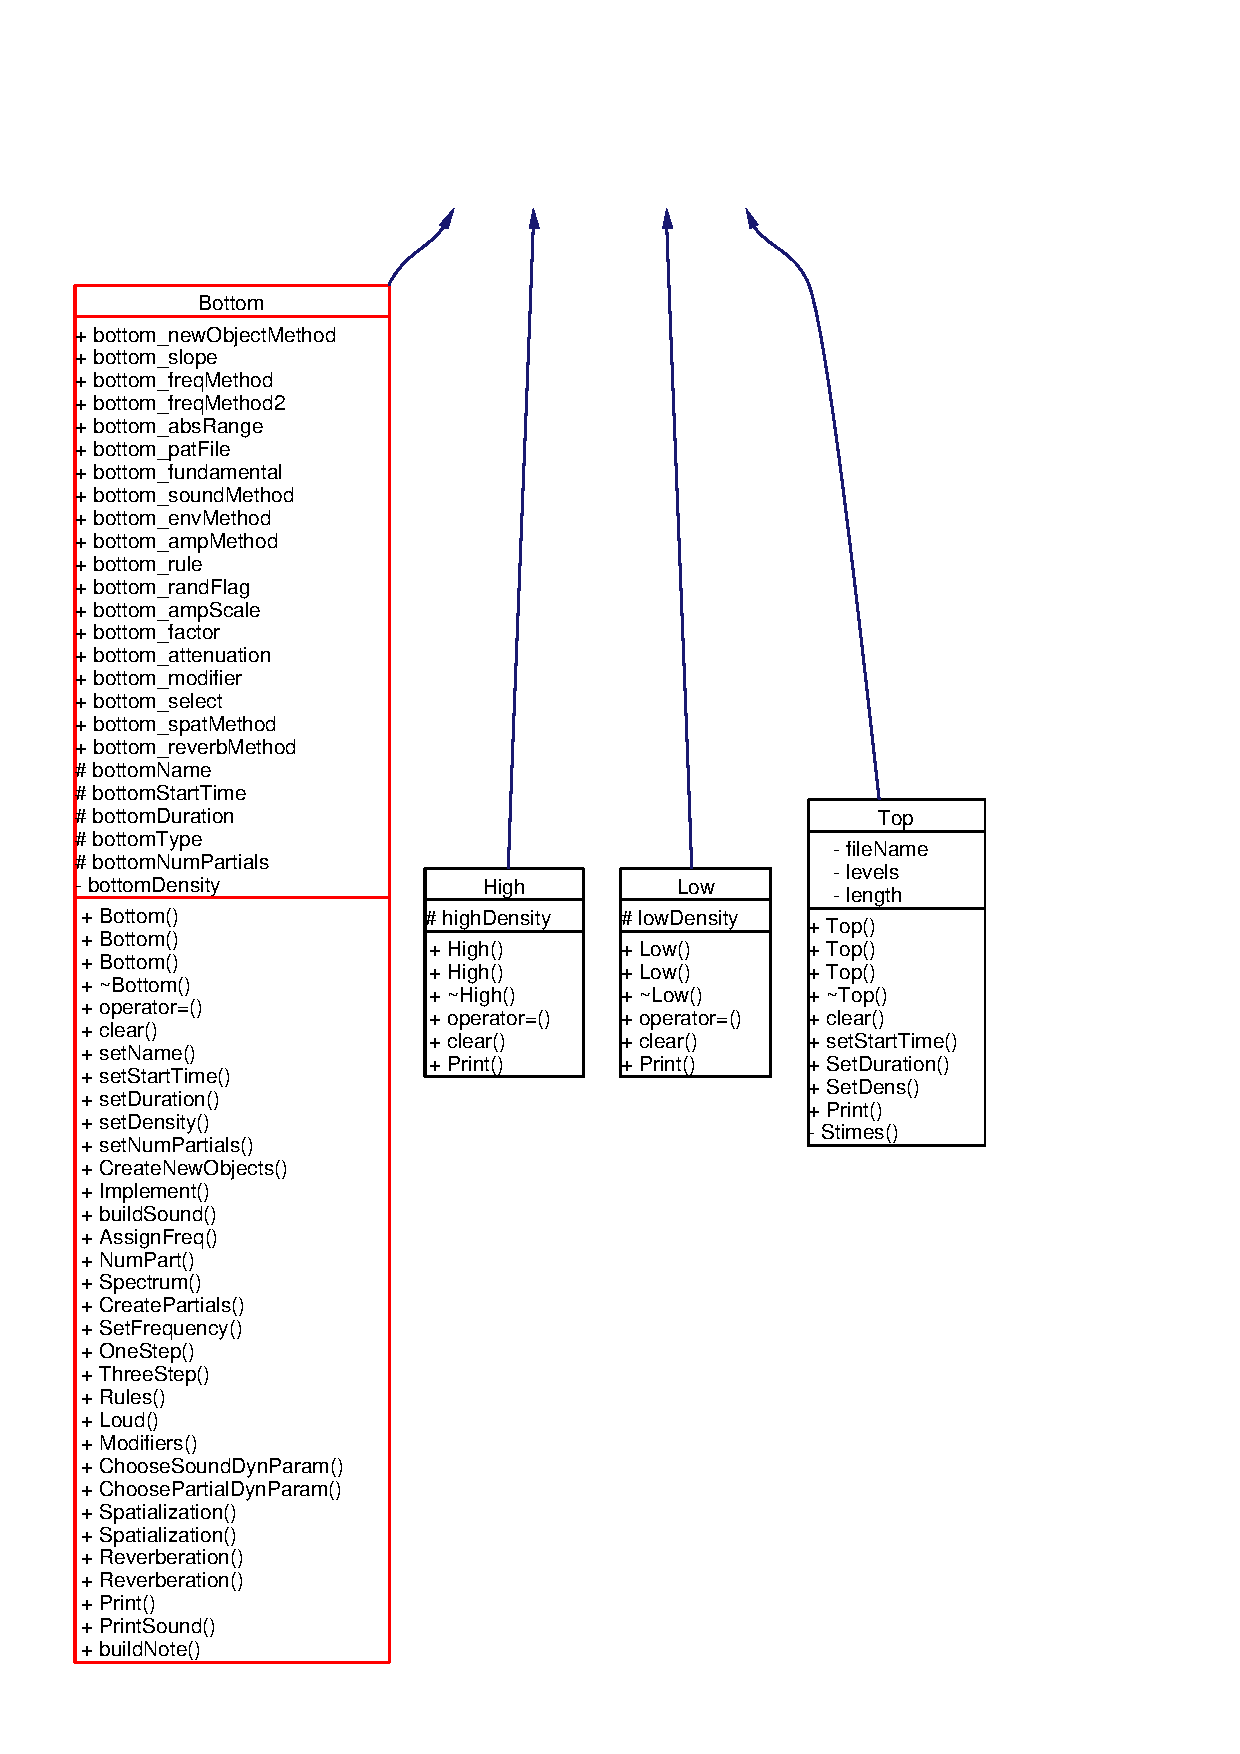
\includegraphics[width=236pt]{classEvent__inherit__graph}
\end{center}
\end{figure}
Collaboration diagram for Event:\begin{figure}[H]
\begin{center}
\leavevmode
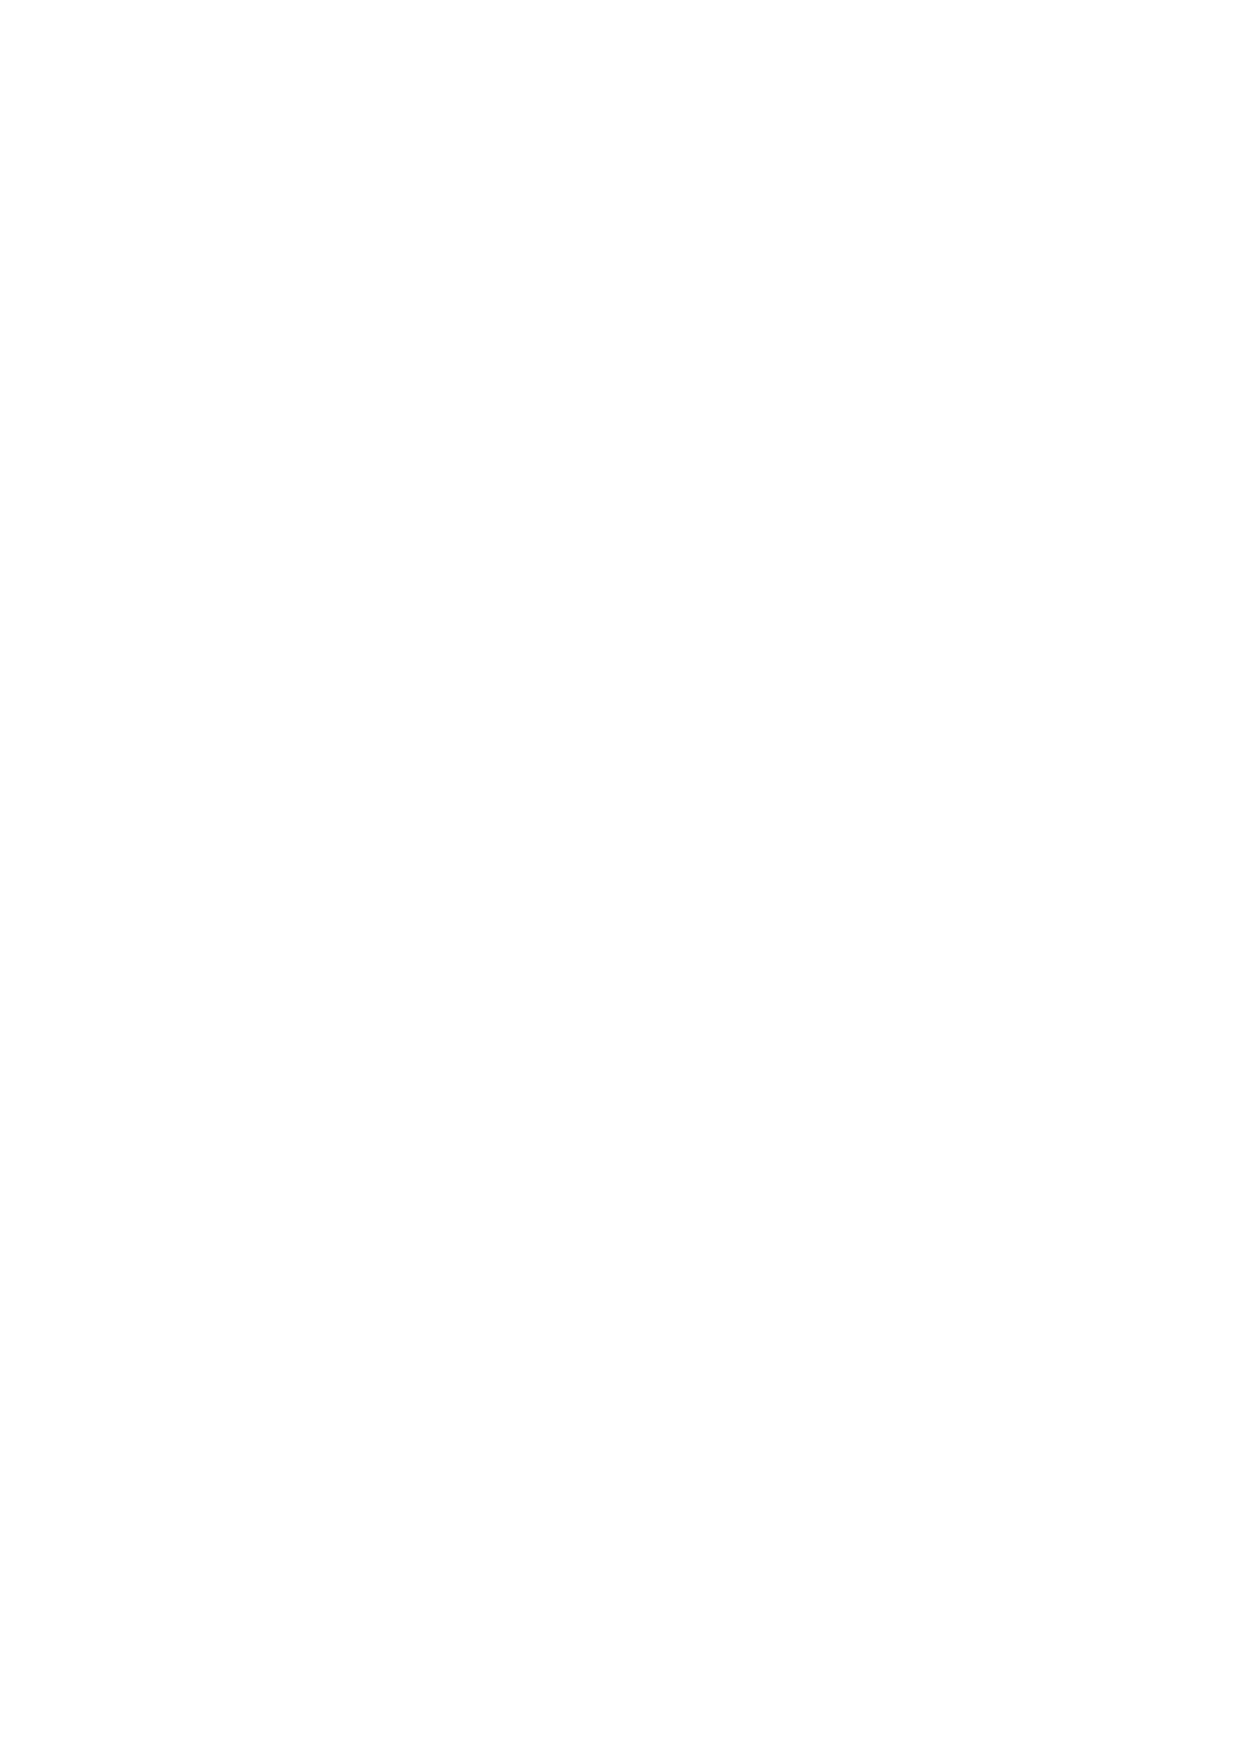
\includegraphics[width=420pt]{classEvent__coll__graph}
\end{center}
\end{figure}
\subsection*{Public Member Functions}
\begin{CompactItemize}
\item 
{\bf Event} ()
\item 
{\bf Event} (char $\ast${\bf a\-Name})
\item 
{\bf Event} (float a\-Start\-Time, float a\-Duration, int a\-Type, char $\ast${\bf a\-Name})
\item 
{\bf Event} (float a\-Start\-Time, float a\-Duration, double a\-Density, int a\-Type, char $\ast${\bf a\-Name})
\item 
{\bf Event} (const  {\bf Event} \&orig\-Event)
\item 
{\bf $\sim$Event} ()
\item 
{\bf Event} \& {\bf operator=} (const  {\bf Event} \&orig\-Event)
\item 
virtual void {\bf set\-Start\-Time} (float a\-Start\-Time)
\item 
virtual void {\bf set\-Duration} (float a\-Duration)
\item 
virtual void {\bf set\-Type} (int a\-Type)
\item 
virtual void {\bf set\-Name} (char $\ast${\bf a\-Name})
\item 
virtual void {\bf set\-Density} (double a\-Density)
\item 
virtual void {\bf clear} ()
\item 
float {\bf get\-Start\-Time} ()
\item 
float {\bf get\-Duration} ()
\item 
char $\ast$ {\bf get\-Name} ()
\item 
double {\bf get\-Density} ()
\item 
int {\bf get\-Type} ()
\item 
int {\bf get\-New\-Obj} ()
\item 
void {\bf Basics} ()
\item 
void {\bf Build} ()
\item 
void {\bf Build} (list$<$ {\bf File\-Value} $>$ data)
\item 
void {\bf Create\-New\-Objects} ()
\item 
void {\bf Build\-Sub\-Events} (map$<$ string, {\bf Event\-Factory} $\ast$ $>$ library, {\bf File\-Value} $\ast$Calculations)
\item 
void {\bf Layer\-Def} ()
\item 
void {\bf New\-Layer\-Def} (list$<$ {\bf File\-Value} $>$ data)
\item 
void {\bf Num\-Objs} ()
\item 
void {\bf New\-Num\-Objs} (list$<$ {\bf File\-Value} $>$ data)
\item 
void {\bf Copy\-Name} ()
\item 
void {\bf New\-Copy\-Name} (list$<$ {\bf File\-Value} $>$ data)
\item 
void {\bf Continuum3} ()
\item 
void {\bf Discrete3} (int slope)
\item 
void {\bf Sweep3} ()
\item 
void {\bf Attack\-Methods} ()
\item 
void {\bf New\-Attack\-Methods} ({\bf File\-Value} args)
\item 
void {\bf Duration\-Methods} ()
\item 
void {\bf New\-Duration\-Methods} ({\bf File\-Value} args)
\item 
void {\bf Attacks} ()
\item 
void {\bf Attacks} (const  char $\ast$e\-Method, vector$<$ int $>$ e\-Arg\-Vector, const  char $\ast$w\-Method, vector$<$ int $>$ w\-Arg\-Vector)
\item 
void {\bf Points\-Probs} ()
\item 
void {\bf Points\-Probs} (const  char $\ast$e\-Method, vector$<$ int $>$ e\-Arg\-Vector, const  char $\ast$w\-Method, vector$<$ int $>$ w\-Arg\-Vector)
\item 
void {\bf Golden\-Mean} ()
\item 
int {\bf Stimes} ()
\item 
void {\bf Durations} ()
\item 
void {\bf Time\-Convert} ()
\item 
void {\bf Select\-Next\-Event} ()
\item 
void {\bf Parameters} (int other\-Params)
\item 
void {\bf set\-Start\-Duration\-Type} (list$<$ {\bf File\-Value} $>$ data)
\item 
void {\bf Continuum} (list$<$ {\bf File\-Value} $>$ data)
\item 
void {\bf Test\-Name\-Type} ()
\item 
void {\bf Create\-Matrices} ()
\item 
void {\bf New\-Create\-Matrices} ({\bf File\-Value} args)
\item 
void {\bf Obj\-Coordinates} ()
\item 
virtual void {\bf build\-Score} (Score $\ast$s)
\item 
void {\bf Adjustments} (int slope)
\item 
int {\bf Find\-Dur} (int remain\-O, float density)
\item 
int {\bf Find\-Len} ()
\item 
virtual void {\bf Print} ()
\item 
virtual void {\bf build\-Note} ()
\item 
double {\bf get\-Check\-Point} ()
\item 
{\bf File\-Value} $\ast$ {\bf get\-Bottom\-Freq} ()
\item 
void {\bf set\-Bottom\-Freq} ({\bf File\-Value} $\ast$s)
\item 
{\bf File\-Value} $\ast$ {\bf get\-Bottom\-Loud} ()
\item 
void {\bf set\-Bottom\-Loud} ({\bf File\-Value} $\ast$s)
\item 
{\bf File\-Value} $\ast$ {\bf get\-Sound\-Num\-Partials} ()
\item 
void {\bf set\-Sound\-Num\-Partials} ({\bf File\-Value} $\ast$s)
\item 
{\bf File\-Value} $\ast$ {\bf get\-Sound\-Deviation} ()
\item 
void {\bf set\-Sound\-Deviation} ({\bf File\-Value} $\ast$s)
\item 
{\bf File\-Value} $\ast$ {\bf get\-Sound\-Part\-Envs} ()
\item 
void {\bf set\-Sound\-Part\-Envs} ({\bf File\-Value} $\ast$s)
\item 
{\bf File\-Value} $\ast$ {\bf get\-Sound\-Modifiers} ()
\item 
void {\bf set\-Sound\-Modifiers} ({\bf File\-Value} $\ast$s)
\item 
{\bf File\-Value} $\ast$ {\bf get\-Sound\-Reverberation} ()
\item 
void {\bf set\-Sound\-Reverberation} ({\bf File\-Value} $\ast$s)
\item 
{\bf File\-Value} $\ast$ {\bf get\-Sound\-Spatialization} ()
\item 
void {\bf set\-Sound\-Spatialization} ({\bf File\-Value} $\ast$s)
\item 
{\bf File\-Value} $\ast$ {\bf get\-Note\-Pitch\-Class} ()
\item 
void {\bf set\-Note\-Pitch\-Class} ({\bf File\-Value} $\ast$s)
\item 
{\bf File\-Value} $\ast$ {\bf get\-Note\-Dynamic\-Mark} ()
\item 
void {\bf set\-Note\-Dynamic\-Mark} ({\bf File\-Value} $\ast$s)
\item 
{\bf File\-Value} $\ast$ {\bf get\-Note\-Modifiers} ()
\item 
void {\bf set\-Note\-Modifiers} ({\bf File\-Value} $\ast$s)
\end{CompactItemize}
\subsection*{Public Attributes}
\begin{CompactItemize}
\item 
double {\bf check\-Point}
\item 
{\bf Matrix} $\ast$ {\bf s0}
\item 
{\bf Matrix} $\ast$ {\bf d0}
\item 
{\bf Matrix} $\ast$ {\bf s1}
\item 
{\bf Matrix} $\ast$ {\bf d1}
\item 
float {\bf the\-Start\-Time}
\item 
float {\bf the\-Duration}
\item 
int {\bf the\-Type}
\item 
char $\ast$ {\bf the\-Name}
\item 
char $\ast$ {\bf a\-Name}
\item 
char $\ast$$\ast$ {\bf name\-Type}
\item 
double {\bf the\-Density}
\item 
list$<$ {\bf Event} $\ast$ $>$ {\bf subevents}
\item 
int {\bf num\-Layers}
\item 
int {\bf obj\-Max\-Dur}
\item 
int {\bf u\-Per\-Sec}
\item 
int {\bf bar\-Len}
\item 
int {\bf max\-Types}
\item 
int {\bf num\-Chars}
\item 
int {\bf levels}
\item 
int {\bf length}
\item 
int {\bf num\-Objs}
\item 
int {\bf obj\-ID}
\item 
int $\ast$ {\bf types\-In\-Layer}
\item 
int {\bf no\-Weights}
\item 
int {\bf array\-Size}
\item 
int {\bf list\-Len}
\item 
int {\bf dur\-Len}
\item 
int $\ast$ {\bf star\-Tarray}
\item 
int $\ast$ {\bf dur\-Array}
\item 
double $\ast$ {\bf prob\-Sieve\-Array}
\item 
double $\ast$ {\bf prob\-Dur\-Array}
\item 
float $\ast$ {\bf layer\-Dens}
\item 
int $\ast$ {\bf objs\-In\-Layer}
\item 
int $\ast$ {\bf remain\-Objs}
\item 
int {\bf dur\-Matrix}
\item 
int {\bf dur\-Units}
\item 
int {\bf stime\-Matrix}
\item 
int {\bf stime\-Units}
\item 
float {\bf dur\-Sec}
\item 
float {\bf stime\-Sec}
\item 
double {\bf du\-Ratio}
\item 
long {\bf loc0}
\item 
long {\bf loc1}
\item 
int {\bf new\-Obj}
\item 
int {\bf type}
\item 
char $\ast$ {\bf keep\-Name}
\item 
int {\bf layer}
\item 
char $\ast$ {\bf fname}
\item 
int {\bf num\-Param}
\item 
float $\ast$ {\bf prob\-Param}
\item 
int $\ast$$\ast$ {\bf data\-Param}
\item 
float $\ast$$\ast$ {\bf coef\-Param}
\item 
int $\ast$$\ast$ {\bf sieve\-Param}
\item 
int $\ast$$\ast$ {\bf temp\-Sieves}
\item 
int $\ast$$\ast$ {\bf max\-Len}
\item 
int $\ast$ {\bf env\-Param}
\item 
float $\ast$ {\bf scale\-Param}
\end{CompactItemize}
\subsection*{Protected Attributes}
\begin{CompactItemize}
\item 
{\bf File\-Value} $\ast$ {\bf bottom\_\-frequency}
\item 
{\bf File\-Value} $\ast$ {\bf bottom\_\-loudness}
\item 
{\bf File\-Value} $\ast$ {\bf sound\_\-num\-Partials}
\item 
{\bf File\-Value} $\ast$ {\bf sound\_\-deviation}
\item 
{\bf File\-Value} $\ast$ {\bf sound\_\-part\-Envs}
\item 
{\bf File\-Value} $\ast$ {\bf sound\_\-modifiers}
\item 
{\bf File\-Value} $\ast$ {\bf sound\_\-reverberation}
\item 
{\bf File\-Value} $\ast$ {\bf sound\_\-spatialization}
\item 
{\bf File\-Value} $\ast$ {\bf note\_\-pitch\-Class}
\item 
{\bf File\-Value} $\ast$ {\bf note\_\-dynamic\-Mark}
\item 
{\bf File\-Value} $\ast$ {\bf note\_\-modifiers}
\item 
float {\bf lastime}
\end{CompactItemize}
\subsection*{Friends}
\begin{CompactItemize}
\item 
class {\bf Matrix}
\end{CompactItemize}


\subsection{Constructor \& Destructor Documentation}
\index{Event@{Event}!Event@{Event}}
\index{Event@{Event}!Event@{Event}}
\subsubsection{\setlength{\rightskip}{0pt plus 5cm}Event::Event ()\hspace{0.3cm}{\tt  [inline]}}\label{classEvent_a0}


Default constructor for an Event. It creates an Event object with no data. 

Definition at line 55 of file event.h.

Referenced by Event().\index{Event@{Event}!Event@{Event}}
\index{Event@{Event}!Event@{Event}}
\subsubsection{\setlength{\rightskip}{0pt plus 5cm}Event::Event (char $\ast$ {\em a\-Name})}\label{classEvent_a1}


Constructor for an Event. Empty event, generic; has only a name. \begin{Desc}
\item[Parameters:]
\begin{description}
\item[{\em a\-Name}]Name of the event \end{description}
\end{Desc}


Definition at line 55 of file event.cpp.

References dur\-Array, layer\-Dens, name\-Type, obj\-ID, objs\-In\-Layer, prob\-Dur\-Array, prob\-Sieve\-Array, remain\-Objs, set\-Name(), star\-Tarray, and types\-In\-Layer.

Here is the call graph for this function:\begin{figure}[H]
\begin{center}
\leavevmode
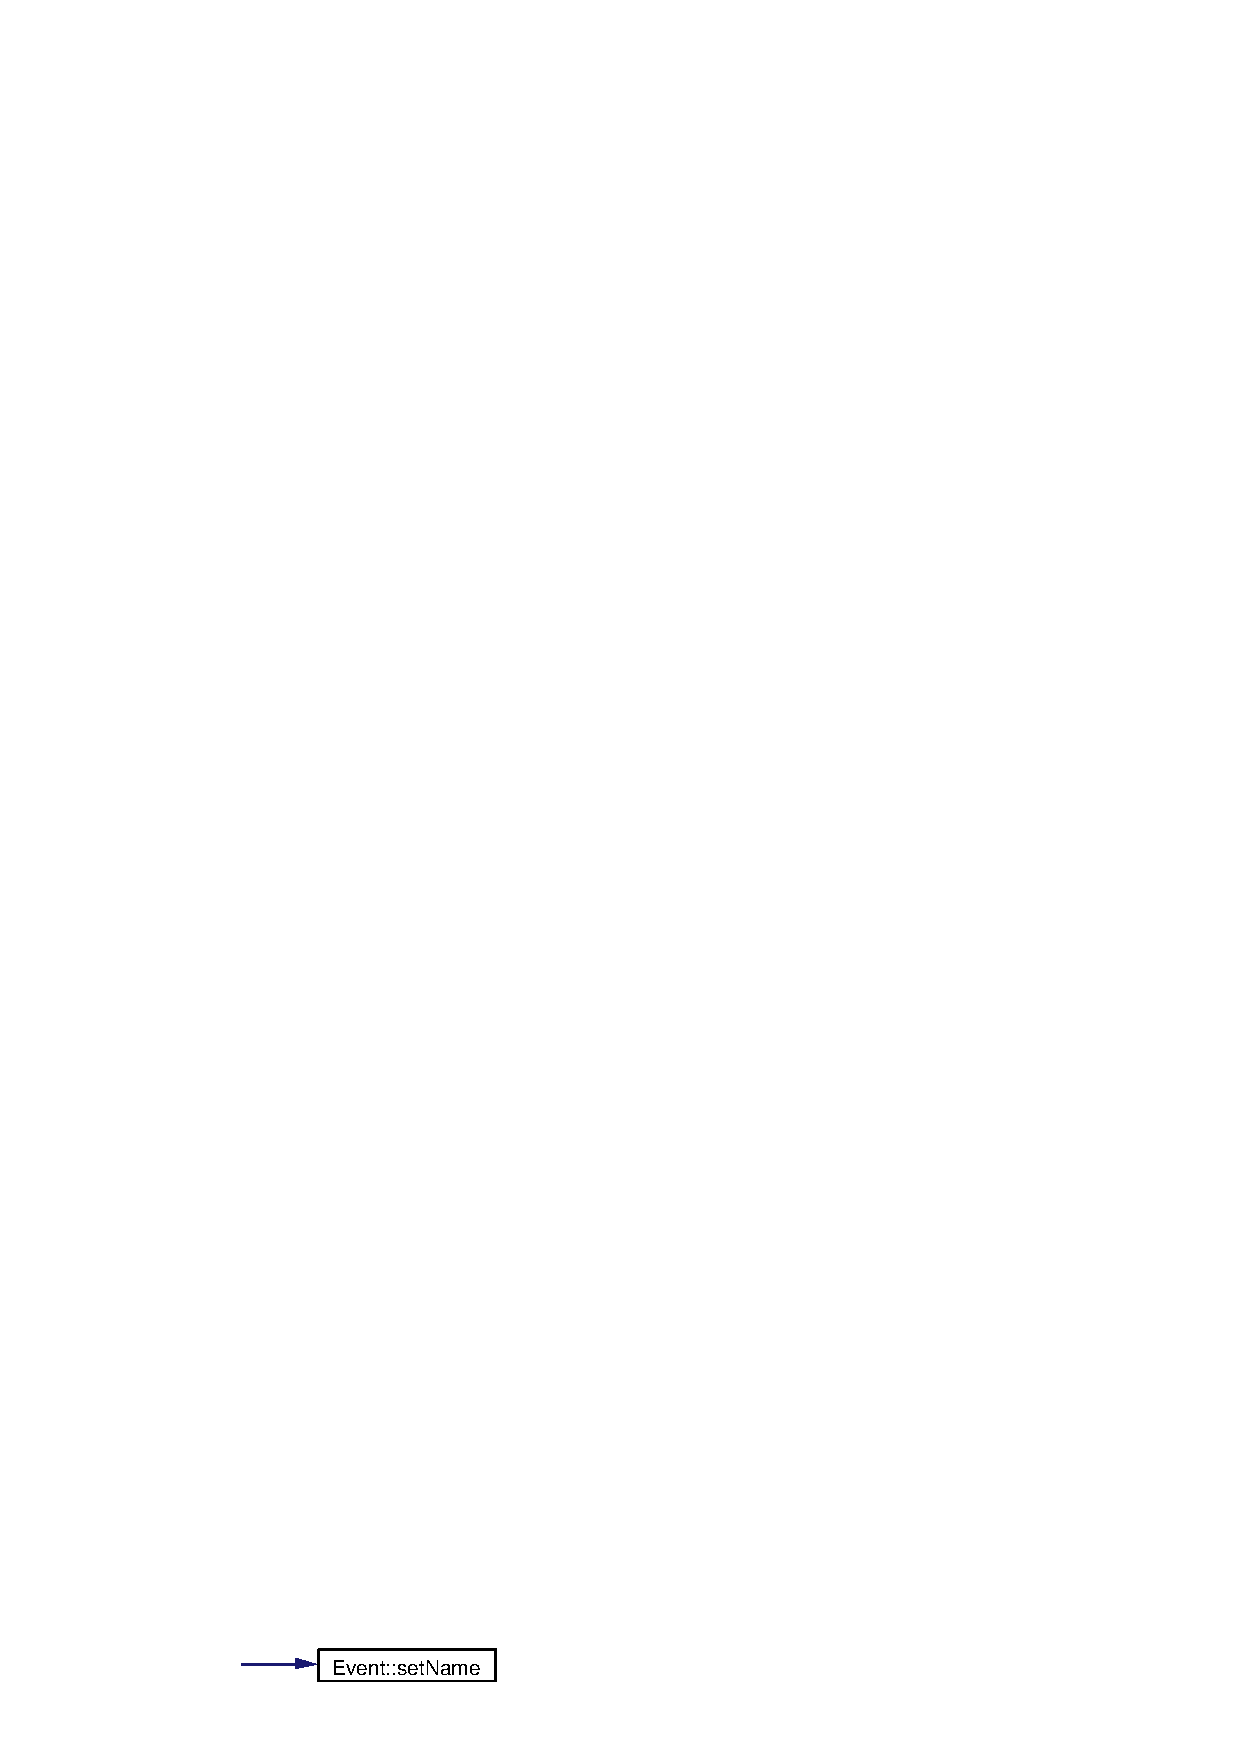
\includegraphics[width=123pt]{classEvent_a1_cgraph}
\end{center}
\end{figure}
\index{Event@{Event}!Event@{Event}}
\index{Event@{Event}!Event@{Event}}
\subsubsection{\setlength{\rightskip}{0pt plus 5cm}Event::Event (float {\em a\-Start\-Time}, float {\em a\-Duration}, int {\em a\-Type}, char $\ast$ {\em a\-Name})}\label{classEvent_a2}


Constructor for an Event. Includes basic information. \begin{Desc}
\item[Parameters:]
\begin{description}
\item[{\em a\-Start\-Time}]Start Time of the event \item[{\em a\-Duration}]Duration of the event \item[{\em a\-Type}]Type of the event \item[{\em Name}]of the event \end{description}
\end{Desc}


Definition at line 78 of file event.cpp.

References dur\-Array, layer\-Dens, name\-Type, obj\-ID, objs\-In\-Layer, prob\-Dur\-Array, prob\-Sieve\-Array, remain\-Objs, set\-Duration(), set\-Name(), set\-Start\-Time(), set\-Type(), star\-Tarray, the\-Density, and types\-In\-Layer.

Here is the call graph for this function:\begin{figure}[H]
\begin{center}
\leavevmode
\includegraphics[width=132pt]{classEvent_a2_cgraph}
\end{center}
\end{figure}
\index{Event@{Event}!Event@{Event}}
\index{Event@{Event}!Event@{Event}}
\subsubsection{\setlength{\rightskip}{0pt plus 5cm}Event::Event (float {\em a\-Start\-Time}, float {\em a\-Duration}, double {\em a\-Density}, int {\em a\-Type}, char $\ast$ {\em a\-Name})}\label{classEvent_a3}


Constructor for an Event. Includes basic information. \begin{Desc}
\item[Parameters:]
\begin{description}
\item[{\em a\-Start\-Time}]Start Time of the event \item[{\em a\-Duration}]Duration of the event \item[{\em a\-Density}]Density of the event \item[{\em a\-Type}]Type of the event \item[{\em Name}]of the event \end{description}
\end{Desc}


Definition at line 102 of file event.cpp.

References Event(), and the\-Density.

Here is the call graph for this function:\begin{figure}[H]
\begin{center}
\leavevmode
\includegraphics[width=116pt]{classEvent_a3_cgraph}
\end{center}
\end{figure}
\index{Event@{Event}!Event@{Event}}
\index{Event@{Event}!Event@{Event}}
\subsubsection{\setlength{\rightskip}{0pt plus 5cm}Event::Event (const {\bf Event} \& {\em orig\-Event})}\label{classEvent_a4}


This is the copy constructor. \begin{Desc}
\item[Parameters:]
\begin{description}
\item[{\em orig\-Event}]Event object to make a copy of \end{description}
\end{Desc}


Definition at line 113 of file event.cpp.

References the\-Density, the\-Duration, the\-Name, and the\-Start\-Time.\index{Event@{Event}!~Event@{$\sim$Event}}
\index{~Event@{$\sim$Event}!Event@{Event}}
\subsubsection{\setlength{\rightskip}{0pt plus 5cm}Event::$\sim${\bf Event} ()}\label{classEvent_a5}


This is the destructor. 

Definition at line 137 of file event.cpp.

References clear().

Here is the call graph for this function:\begin{figure}[H]
\begin{center}
\leavevmode
\includegraphics[width=116pt]{classEvent_a5_cgraph}
\end{center}
\end{figure}


\subsection{Member Function Documentation}
\index{Event@{Event}!Adjustments@{Adjustments}}
\index{Adjustments@{Adjustments}!Event@{Event}}
\subsubsection{\setlength{\rightskip}{0pt plus 5cm}void Event::Adjustments (int {\em slope})}\label{classEvent_a54}


Works only on the s0 (attacks/types matrix). Find the layer this obj\-Type belongs to. Determine the duration of this obj. Adjust the vector and matrix; get them ready for next choice. The sizes of stime\-Matrix and dur\-Matrix are measured in number of entries in the matrix while end\-Units\-M is measured in basic units (pulses, not seconds). \begin{Desc}
\item[Parameters:]
\begin{description}
\item[{\em slope}]Slope value to pass to Adjust\-Matrix() \end{description}
\end{Desc}


Definition at line 1151 of file event.cpp.

References Matrix::Adjust\-Matrix(), Matrix::Adjust\-Vector(), Find\-Dur(), layer, layer\-Dens, new\-Obj, num\-Layers, num\-Objs, remain\-Objs, s0, stime\-Matrix, type, and types\-In\-Layer.

Referenced by Discrete3().

Here is the call graph for this function:\begin{figure}[H]
\begin{center}
\leavevmode
\includegraphics[width=301pt]{classEvent_a54_cgraph}
\end{center}
\end{figure}
\index{Event@{Event}!AttackMethods@{AttackMethods}}
\index{AttackMethods@{AttackMethods}!Event@{Event}}
\subsubsection{\setlength{\rightskip}{0pt plus 5cm}void Event::Attack\-Methods ()}\label{classEvent_a33}


Choosing a method to determine attack times 

\begin{Desc}
\item[{\bf Deprecated}]Use {\bf New\-Attack\-Methods()}{\rm (p.\,\pageref{classEvent_a34})} with the new interface \end{Desc}
\index{Event@{Event}!Attacks@{Attacks}}
\index{Attacks@{Attacks}!Event@{Event}}
\subsubsection{\setlength{\rightskip}{0pt plus 5cm}void Event::Attacks (const char $\ast$ {\em e\-Method}, vector$<$ int $>$ {\em e\-Arg\-Vector}, const char $\ast$ {\em w\-Method}, vector$<$ int $>$ {\em w\-Arg\-Vector})}\label{classEvent_a38}


Creates an array (sieve) with all possible attacks and another array with their probabilities. \begin{Desc}
\item[Parameters:]
\begin{description}
\item[{\em e\-Method}]e-Method for {\bf Sieve}{\rm (p.\,\pageref{classSieve})} \item[{\em e\-Arg\-Vector}]e-Vector for {\bf Sieve}{\rm (p.\,\pageref{classSieve})} \item[{\em w\-Method}]w-Method for {\bf Sieve}{\rm (p.\,\pageref{classSieve})} \item[{\em w\-Arg\-Vector}]w-Vector for {\bf Sieve}{\rm (p.\,\pageref{classSieve})} \end{description}
\end{Desc}


Definition at line 889 of file event.cpp.

References array\-Size, Sieve::Build(), Sieve::Fill\-In\-Arrays(), Sieve::Get\-List\-Len(), list\-Len, prob\-Sieve\-Array, star\-Tarray, the\-Duration, and u\-Per\-Sec.

Here is the call graph for this function:\begin{figure}[H]
\begin{center}
\leavevmode
\includegraphics[width=291pt]{classEvent_a38_cgraph}
\end{center}
\end{figure}
\index{Event@{Event}!Attacks@{Attacks}}
\index{Attacks@{Attacks}!Event@{Event}}
\subsubsection{\setlength{\rightskip}{0pt plus 5cm}void Event::Attacks ()}\label{classEvent_a37}


Creates an array (sieve) with all possible attacks and another array with their probabilities. 

\begin{Desc}
\item[{\bf Deprecated}]Not in use (use Attacks(char$\ast$, vector$<$int$>$, char$\ast$, vector$<$int$>$) instead) \end{Desc}


Referenced by New\-Attack\-Methods().\index{Event@{Event}!Basics@{Basics}}
\index{Basics@{Basics}!Event@{Event}}
\subsubsection{\setlength{\rightskip}{0pt plus 5cm}void Event::Basics ()}\label{classEvent_a19}


Chooses the values needed for start time, type, and duration. 

\begin{Desc}
\item[{\bf Deprecated}]\end{Desc}
\index{Event@{Event}!Build@{Build}}
\index{Build@{Build}!Event@{Event}}
\subsubsection{\setlength{\rightskip}{0pt plus 5cm}void Event::Build (list$<$ {\bf File\-Value} $>$ {\em data})}\label{classEvent_a21}


Builds the event by calling a series of functions and determining: the number of streams/layers in this event; the number of objects in each layer; the names of the files describing the objects contained in this event. \begin{Desc}
\item[Parameters:]
\begin{description}
\item[{\em data}]A list of file values to build the event. \end{description}
\end{Desc}


Definition at line 380 of file event.cpp.

References New\-Copy\-Name(), New\-Layer\-Def(), and New\-Num\-Objs().

Here is the call graph for this function:\begin{figure}[H]
\begin{center}
\leavevmode
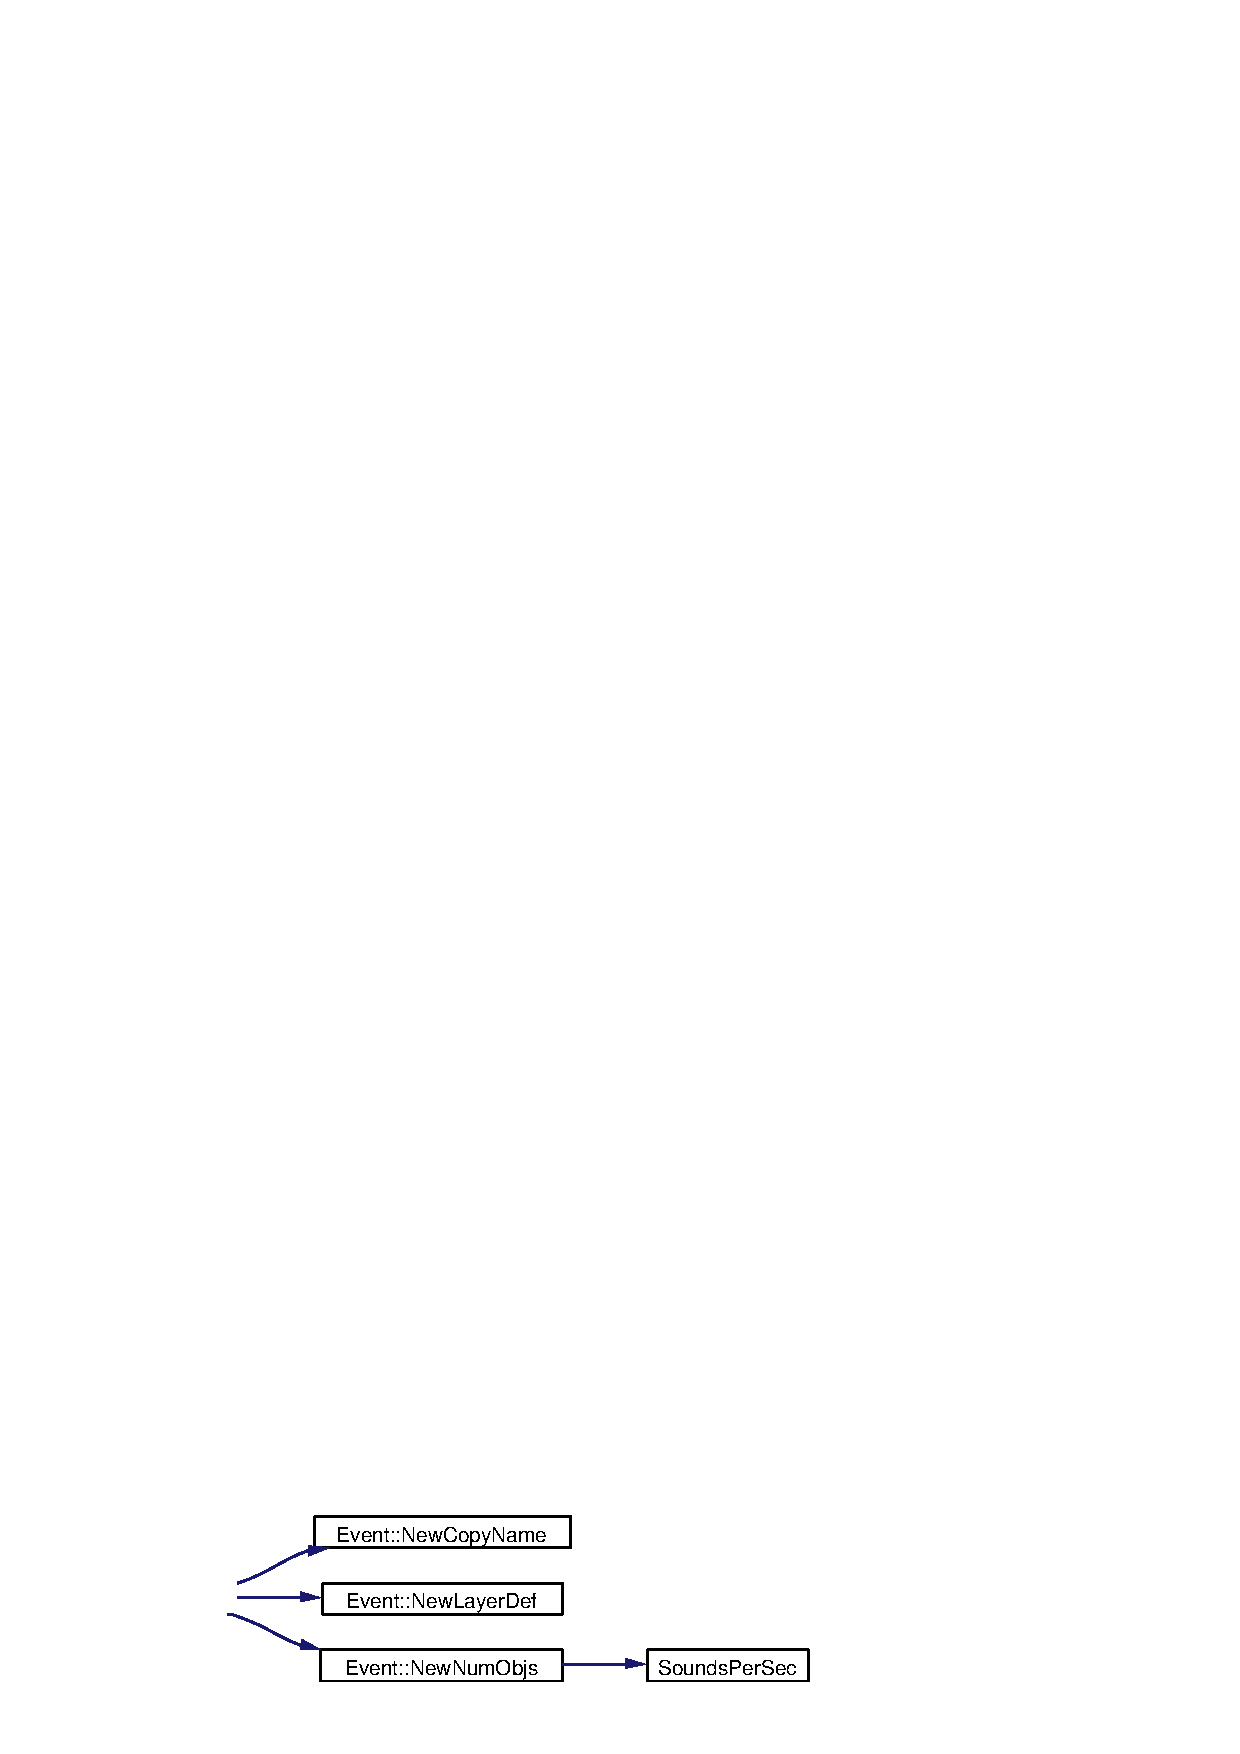
\includegraphics[width=198pt]{classEvent_a21_cgraph}
\end{center}
\end{figure}
\index{Event@{Event}!Build@{Build}}
\index{Build@{Build}!Event@{Event}}
\subsubsection{\setlength{\rightskip}{0pt plus 5cm}void Event::Build ()}\label{classEvent_a20}


Builds the event by calling a series of functions and determining: the number of streams/layers in this event; the number of objects in each layer; the names of the files describing the objects contained in this event. 

\begin{Desc}
\item[{\bf Deprecated}]Use {\bf Build(list$<$File\-Value$>$ data)}{\rm (p.\,\pageref{classEvent_a21})} instead \end{Desc}
\index{Event@{Event}!buildNote@{buildNote}}
\index{buildNote@{buildNote}!Event@{Event}}
\subsubsection{\setlength{\rightskip}{0pt plus 5cm}void Event::build\-Note ()\hspace{0.3cm}{\tt  [virtual]}}\label{classEvent_a58}




Reimplemented in {\bf Bottom} {\rm (p.\,\pageref{classBottom_a32})}.

Definition at line 2038 of file event.cpp.

References Print(), and subevents.

Referenced by Bottom::build\-Note(), and Build\-Sub\-Events().

Here is the call graph for this function:\begin{figure}[H]
\begin{center}
\leavevmode
\includegraphics[width=123pt]{classEvent_a58_cgraph}
\end{center}
\end{figure}
\index{Event@{Event}!buildScore@{buildScore}}
\index{buildScore@{buildScore}!Event@{Event}}
\subsubsection{\setlength{\rightskip}{0pt plus 5cm}void Event::build\-Score (Score $\ast$ {\em s})\hspace{0.3cm}{\tt  [virtual]}}\label{classEvent_a53}




Definition at line 2028 of file event.cpp.

References subevents.\index{Event@{Event}!BuildSubEvents@{BuildSubEvents}}
\index{BuildSubEvents@{BuildSubEvents}!Event@{Event}}
\subsubsection{\setlength{\rightskip}{0pt plus 5cm}void Event::Build\-Sub\-Events (map$<$ string, {\bf Event\-Factory} $\ast$ $>$ {\em library}, {\bf File\-Value} $\ast$ {\em Calculations})}\label{classEvent_a23}


Build\-Sub\-Events. Taken from Create\-New\-Objects. Build sub-events from parsed information and information already set for this event. --- To be used with new interface.--- \begin{Desc}
\item[Parameters:]
\begin{description}
\item[{\em library}]XXXXXXXXXXXXXXXXXXX \item[{\em Calculations}]YYYYYYYYYYYYY \end{description}
\end{Desc}


Definition at line 1459 of file event.cpp.

References Event\-Factory::Build(), build\-Note(), Bottom::build\-Sound(), check\-Point, Discrete3(), dur\-Sec, File\-Value::Evaluate(), File\-Value::get\-List\-Ptr(), File\-Value::get\-Number(), File\-Value::get\-String(), Event\-Factory::Inherit(), lastime, loc0, name\-Type, New\-Attack\-Methods(), New\-Create\-Matrices(), New\-Duration\-Methods(), new\-Obj, num\-Objs, obj\-ID, score, sever, stime\-Sec, subevents, the\-Duration, the\-Name, type, and u\-Per\-Sec.

Referenced by Event\-Factory::Build().

Here is the call graph for this function:\begin{figure}[H]
\begin{center}
\leavevmode
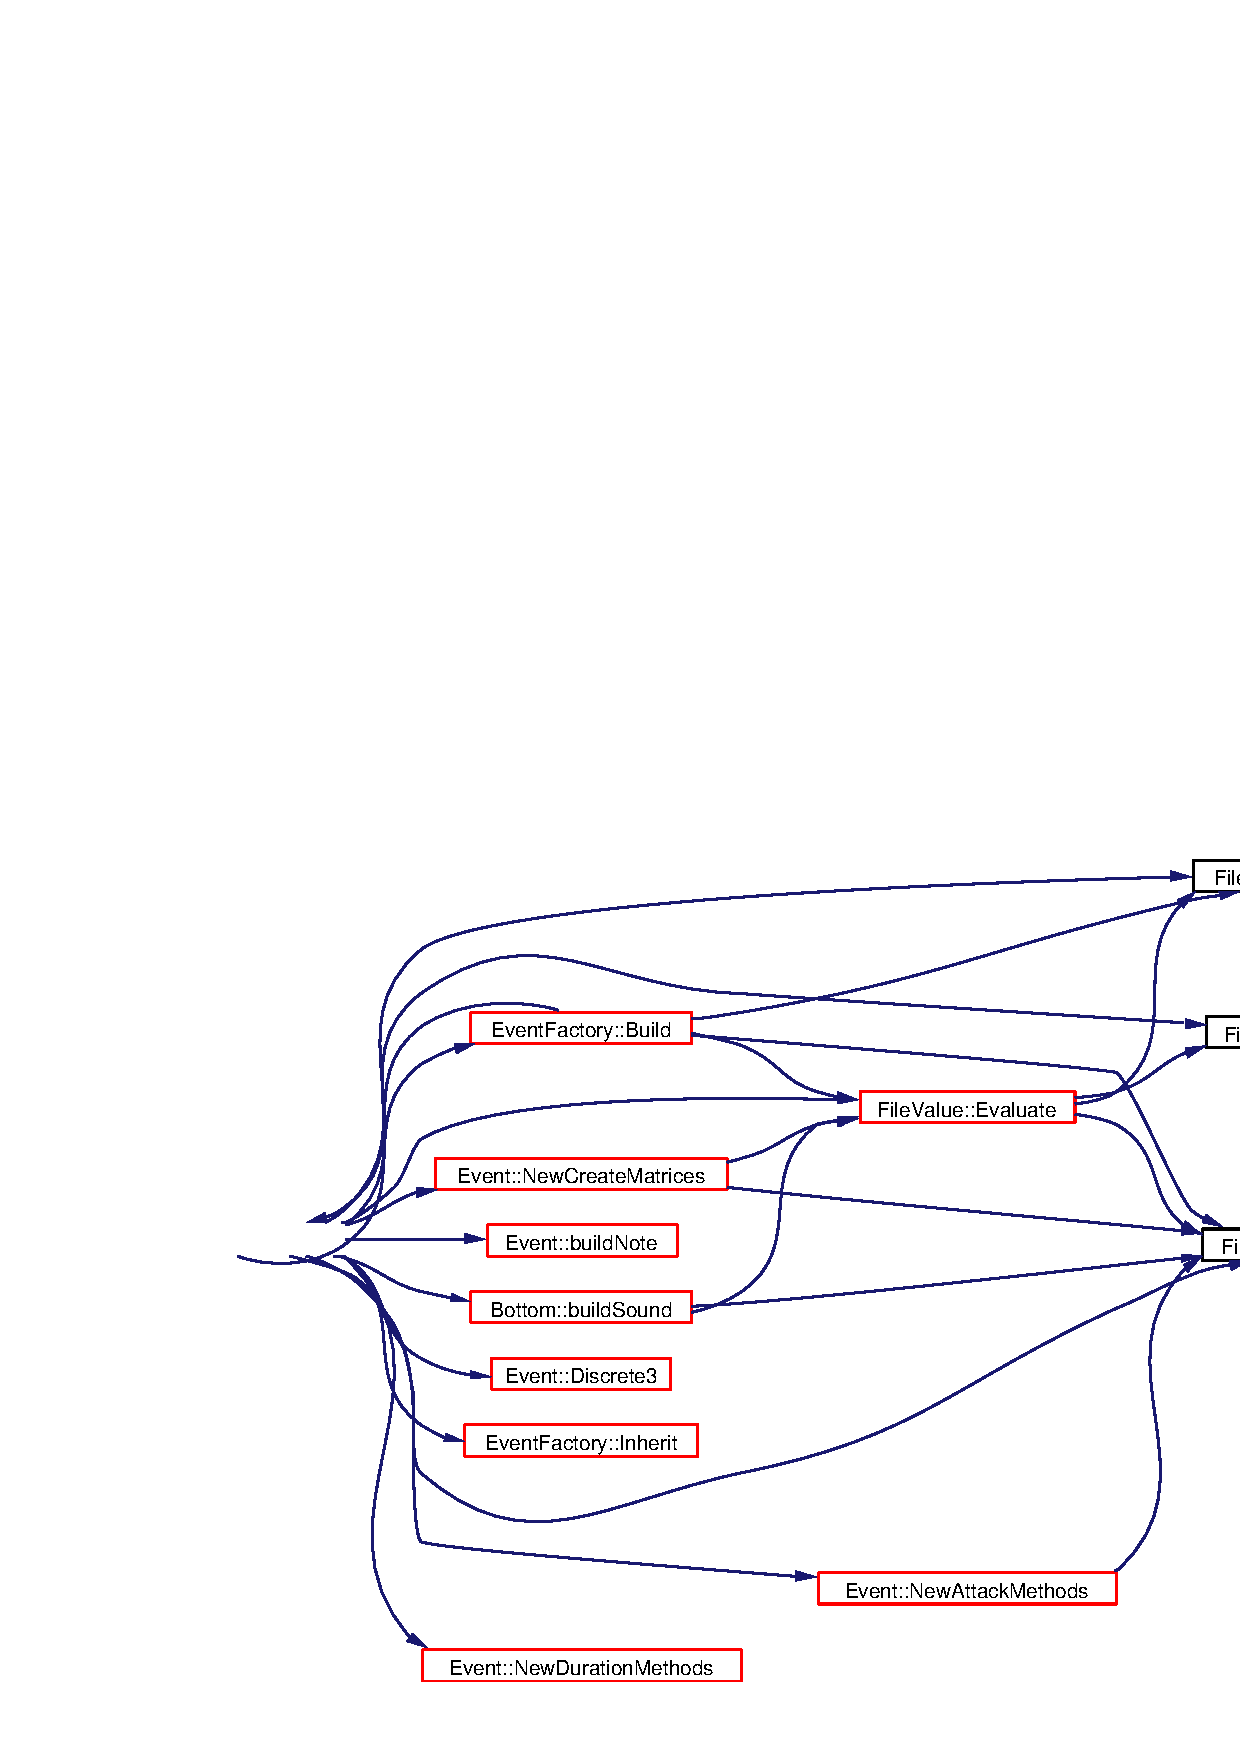
\includegraphics[width=349pt]{classEvent_a23_cgraph}
\end{center}
\end{figure}
\index{Event@{Event}!clear@{clear}}
\index{clear@{clear}!Event@{Event}}
\subsubsection{\setlength{\rightskip}{0pt plus 5cm}void Event::clear ()\hspace{0.3cm}{\tt  [virtual]}}\label{classEvent_a12}


Clears several internal structures in the Event: name\-Type, max\-Types, layer\-Dens, objs\-In\-Layer, remain\-Objs, types\-In\-Layer, star\-Tarray, prob\-Sieve\-Array, dur\-Array, prob\-Dur\-Array 

Reimplemented in {\bf Bottom} {\rm (p.\,\pageref{classBottom_a5})}, {\bf High} {\rm (p.\,\pageref{classHigh_a4})}, {\bf Low} {\rm (p.\,\pageref{classLow_a4})}, {\bf Note} {\rm (p.\,\pageref{classNote_a14})}, and {\bf Top} {\rm (p.\,\pageref{classTop_a4})}.

Definition at line 147 of file event.cpp.

References dur\-Array, layer\-Dens, max\-Types, name\-Type, objs\-In\-Layer, prob\-Dur\-Array, prob\-Sieve\-Array, remain\-Objs, star\-Tarray, and types\-In\-Layer.

Referenced by $\sim$Event().\index{Event@{Event}!Continuum@{Continuum}}
\index{Continuum@{Continuum}!Event@{Event}}
\subsubsection{\setlength{\rightskip}{0pt plus 5cm}void Event::Continuum (list$<$ {\bf File\-Value} $>$ {\em data})}\label{classEvent_a48}


\begin{Desc}
\item[{\bf Deprecated}]DO NOT USE \end{Desc}


Definition at line 1723 of file event.cpp.

References check\-Point, dur\-Sec, obj\-Max\-Dur, stime\-Sec, the\-Duration, type, and u\-Per\-Sec.\index{Event@{Event}!Continuum3@{Continuum3}}
\index{Continuum3@{Continuum3}!Event@{Event}}
\subsubsection{\setlength{\rightskip}{0pt plus 5cm}void Event::Continuum3 ()}\label{classEvent_a30}


DEPRECATED

Continuum3. Method for assigning values for stime\-Sec, and duration using continuous (stochastic) distributions and for type - actually, a discrete value.. 

Definition at line 1691 of file event.cpp.

References check\-Point, Choose\-Offset(), dur\-Sec, new\-Obj, obj\-Max\-Dur, Random::Rand(), Read\-Compute\-Float(), Read\-Compute\-Int(), stime\-Sec, the\-Duration, type, and u\-Per\-Sec.

Here is the call graph for this function:\begin{figure}[H]
\begin{center}
\leavevmode
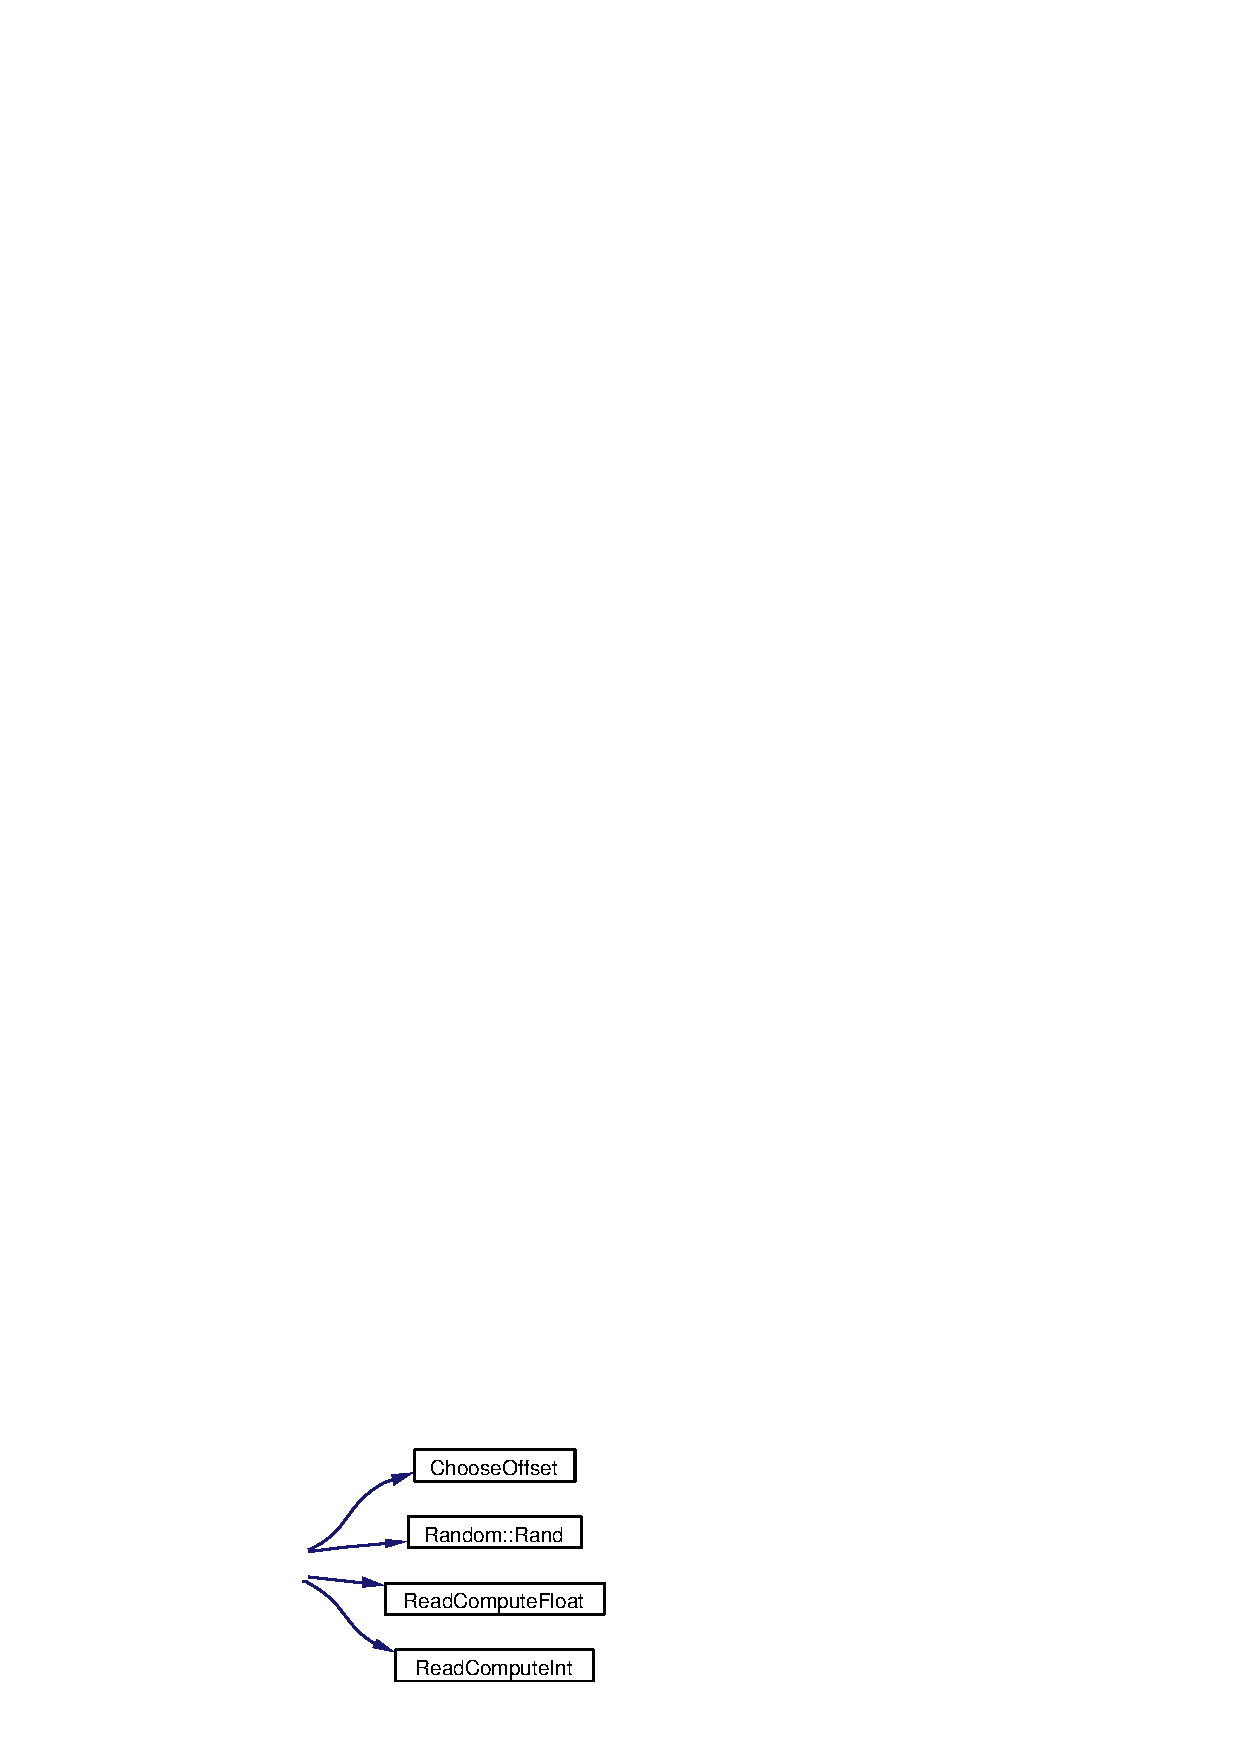
\includegraphics[width=149pt]{classEvent_a30_cgraph}
\end{center}
\end{figure}
\index{Event@{Event}!CopyName@{CopyName}}
\index{CopyName@{CopyName}!Event@{Event}}
\subsubsection{\setlength{\rightskip}{0pt plus 5cm}void Event::Copy\-Name ()}\label{classEvent_a28}


Reads the names of the files defining the elements of the next level and stores them in the two dimenssional character array Name\-Type. 

\begin{Desc}
\item[{\bf Deprecated}]Use New\-Copy\-Name instead \end{Desc}


Definition at line 605 of file event.cpp.

References Data\-In::int\-Vect, max\-Types, Data\-In::name\-Of, name\-Type, num\-Chars, Data\-In::Read\-Chars(), Data\-In::Read\-Dummies(), and Data\-In::Read\-Ints().

Here is the call graph for this function:\begin{figure}[H]
\begin{center}
\leavevmode
\includegraphics[width=154pt]{classEvent_a28_cgraph}
\end{center}
\end{figure}
\index{Event@{Event}!CreateMatrices@{CreateMatrices}}
\index{CreateMatrices@{CreateMatrices}!Event@{Event}}
\subsubsection{\setlength{\rightskip}{0pt plus 5cm}void Event::Create\-Matrices ()}\label{classEvent_a50}


\begin{Desc}
\item[{\bf Deprecated}]DO NOT USE: Use {\bf New\-Create\-Matrices()}{\rm (p.\,\pageref{classEvent_a51})} instead \end{Desc}
\index{Event@{Event}!CreateNewObjects@{CreateNewObjects}}
\index{CreateNewObjects@{CreateNewObjects}!Event@{Event}}
\subsubsection{\setlength{\rightskip}{0pt plus 5cm}void Event::Create\-New\-Objects ()}\label{classEvent_a22}


Contains a loop whthin which objects arec created one at a time. Each object has at least three parameters: start time, duration, and type. They are selected using one of the following methods: CONTINUUM for continuous probability, non-sequential order DISCRETE for discrete values, using a {\bf Matrix}{\rm (p.\,\pageref{classMatrix})} object, non-sequential SWEEP for reading values from a file provided by the user, sequential order 

\begin{Desc}
\item[{\bf Deprecated}]Not currently in use (no replacement) \end{Desc}


Reimplemented in {\bf Bottom} {\rm (p.\,\pageref{classBottom_a11})}.\index{Event@{Event}!Discrete3@{Discrete3}}
\index{Discrete3@{Discrete3}!Event@{Event}}
\subsubsection{\setlength{\rightskip}{0pt plus 5cm}void Event::Discrete3 (int {\em slope})}\label{classEvent_a31}


Sweep. Method for assigning stime\-Sec and dur\-Sec values in sequential order - \char`\"{}sweepeing\char`\"{} from left to right or beginning to end of the event. For stime and duration two different methods are used, one for integer values the other for float values. Type being a discrete value, the integer values method is used for it. $\ast$$\ast$ For use with new interface $\ast$$\ast$ 

Definition at line 1872 of file event.cpp.

References Adjustments(), Obj\-Coordinates(), and Time\-Convert().

Referenced by Build\-Sub\-Events().

Here is the call graph for this function:\begin{figure}[H]
\begin{center}
\leavevmode
\includegraphics[width=365pt]{classEvent_a31_cgraph}
\end{center}
\end{figure}
\index{Event@{Event}!DurationMethods@{DurationMethods}}
\index{DurationMethods@{DurationMethods}!Event@{Event}}
\subsubsection{\setlength{\rightskip}{0pt plus 5cm}void Event::Duration\-Methods ()}\label{classEvent_a35}


Choosing a method to determine durations. 

\begin{Desc}
\item[{\bf Deprecated}]Use {\bf New\-Duration\-Methods()}{\rm (p.\,\pageref{classEvent_a36})} with the new interface \end{Desc}


Definition at line 749 of file event.cpp.

References List$<$ Etype $>$::Insert\-In\-Order(), Data\-In::name\-Of, Points\-Probs(), Data\-In::Read\-Chars(), Data\-In::Read\-Dummies(), and sever.

Here is the call graph for this function:\begin{figure}[H]
\begin{center}
\leavevmode
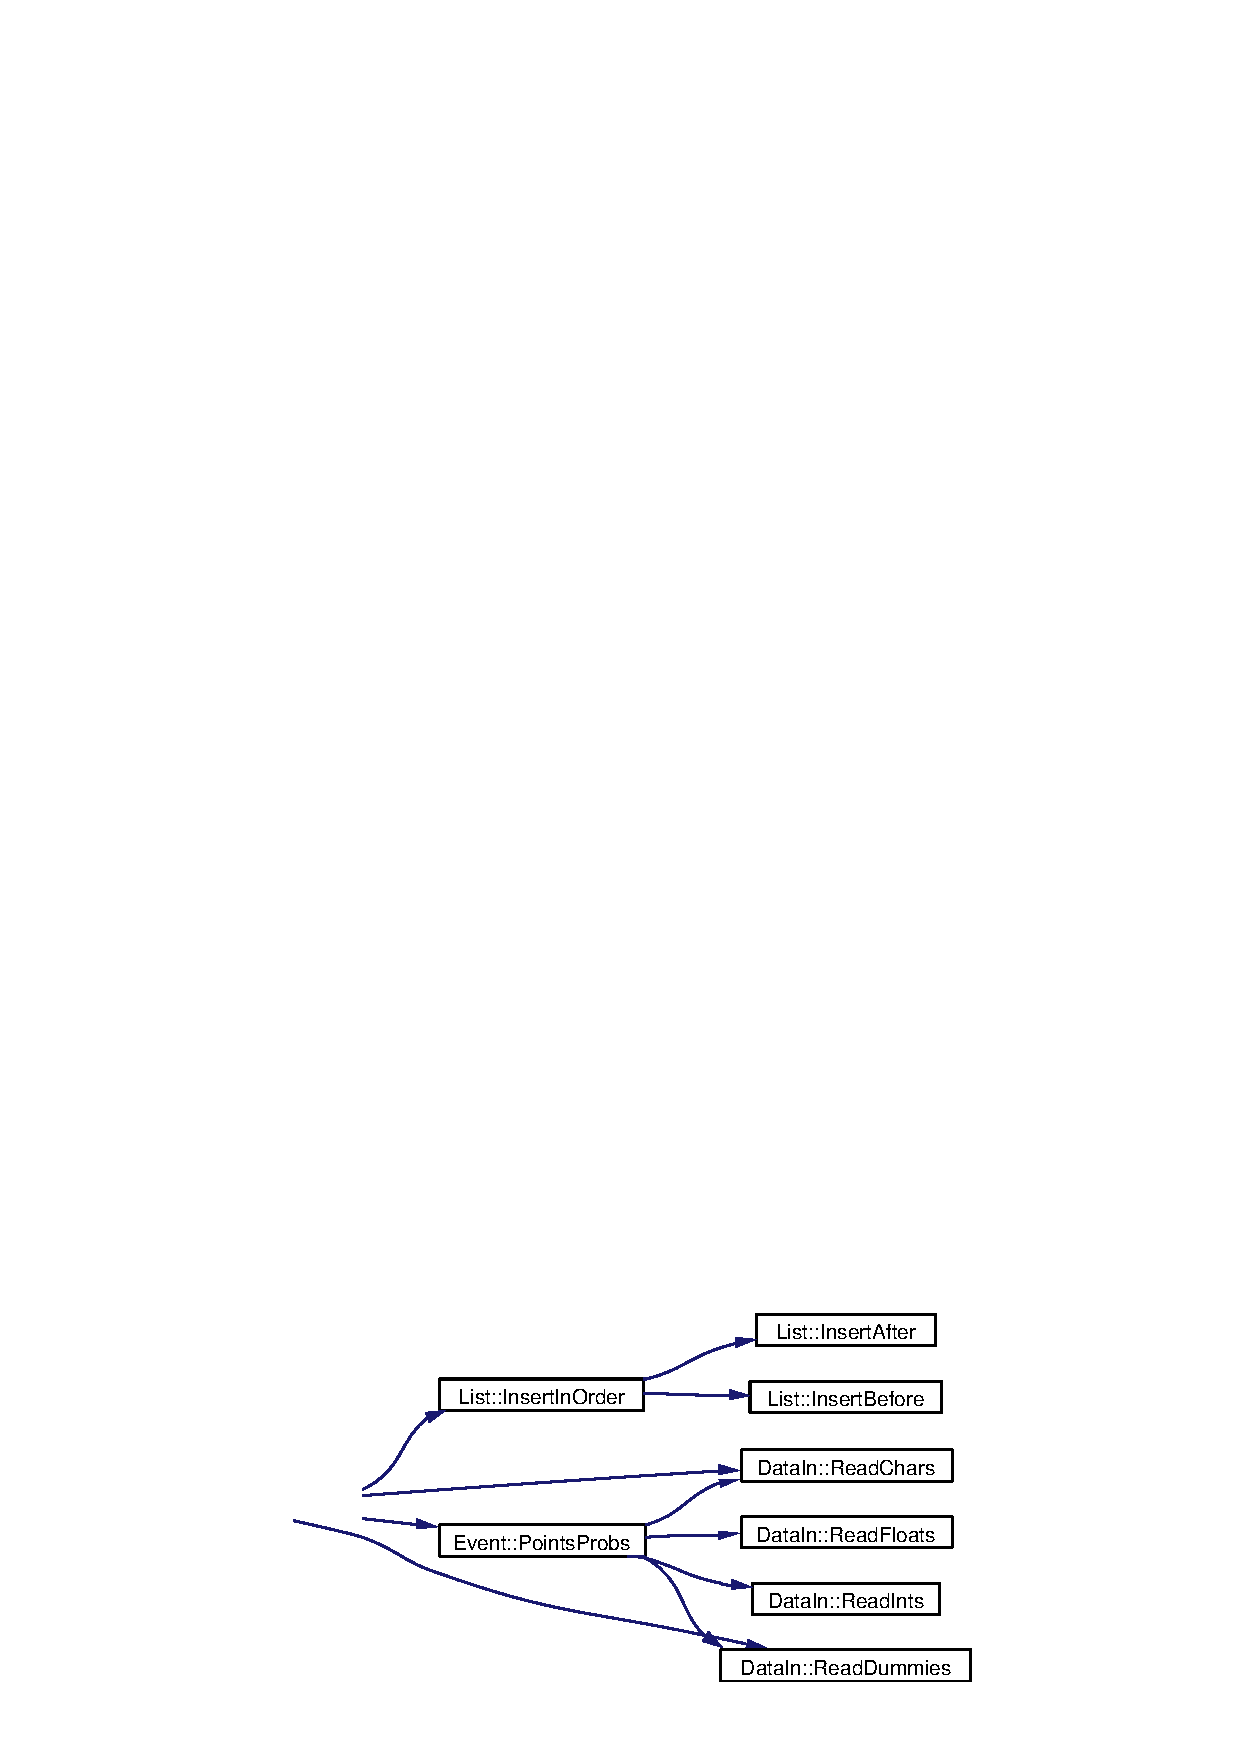
\includegraphics[width=237pt]{classEvent_a35_cgraph}
\end{center}
\end{figure}
\index{Event@{Event}!Durations@{Durations}}
\index{Durations@{Durations}!Event@{Event}}
\subsubsection{\setlength{\rightskip}{0pt plus 5cm}void Event::Durations ()}\label{classEvent_a43}


\begin{Desc}
\item[{\bf Deprecated}]NOT IMPLEMENTED - DO NOT USE \end{Desc}
\index{Event@{Event}!FindDur@{FindDur}}
\index{FindDur@{FindDur}!Event@{Event}}
\subsubsection{\setlength{\rightskip}{0pt plus 5cm}int Event::Find\-Dur (int {\em remain\-O}, float {\em density})}\label{classEvent_a55}


Finds the available space (dur\-Loc) in the matrix for the next duration (max lenght for the next dur starting at this stime\-Matrix). Copies the original duration matrix and adjusts it; selects a duration for this obj type, at this stime\-Matrix. stime\-Matrix, dur\-Matrix, and end\-Loc\-M are expressed in matrix locations; end\-Units\-M is expressed in basic units (pulses). Units: the\-Duration - seconds end\-Units\-M, star\-Tarray[stime\-Matrix], dur\-Array[location] - units (pulses) dur\-Loc, list\-Len, dur\-Len, stime\-Matrix, dur\-Matrix, star\-Tarray, tryloc, dur\-Array - array locations \begin{Desc}
\item[Parameters:]
\begin{description}
\item[{\em remain0}]... \item[{\em density}]... \end{description}
\end{Desc}


Definition at line 1213 of file event.cpp.

References Matrix::Choose\-M(), d0, d1, dur\-Array, dur\-Matrix, Find\-Len(), list\-Len, Matrix, Matrix::Mult(), Matrix::Normalize(), Matrix::row, star\-Tarray, stime\-Matrix, Matrix::Trim\-Matrix(), and type.

Referenced by Adjustments().

Here is the call graph for this function:\begin{figure}[H]
\begin{center}
\leavevmode
\includegraphics[width=214pt]{classEvent_a55_cgraph}
\end{center}
\end{figure}
\index{Event@{Event}!FindLen@{FindLen}}
\index{FindLen@{FindLen}!Event@{Event}}
\subsubsection{\setlength{\rightskip}{0pt plus 5cm}int Event::Find\-Len ()}\label{classEvent_a56}


Find\-Len. Finds the matrix location where the event ends (end\-Loc\-M). star\-Tarray: array of possible start times (in units) stime\-Matrix: a location in star\-Tarray (locations) dur\-Array: array of possible durations (in units) dur\-Len: cardinal of durr\-Array (locations) dur\-Loc: a location in durr\-Array (locations) the\-Duration: total duration of parent event (in seconds) u\-Per\-Sec: number of units in a second end\-Units\-M: the end of the event (in units) test\-End: the end of the event (locations) 

Definition at line 1266 of file event.cpp.

References dur\-Array, dur\-Len, list\-Len, Matrix::matrix, s0, star\-Tarray, stime\-Matrix, the\-Duration, type, and u\-Per\-Sec.

Referenced by Find\-Dur().\index{Event@{Event}!getBottomFreq@{getBottomFreq}}
\index{getBottomFreq@{getBottomFreq}!Event@{Event}}
\subsubsection{\setlength{\rightskip}{0pt plus 5cm}{\bf File\-Value}$\ast$ Event::get\-Bottom\-Freq ()\hspace{0.3cm}{\tt  [inline]}}\label{classEvent_a60}


Get bottom frequency \begin{Desc}
\item[Returns:]A {\bf File\-Value}{\rm (p.\,\pageref{classFileValue})} $\ast$ to the bottom frequency of the event \end{Desc}


Definition at line 541 of file event.h.

References bottom\_\-frequency.

Referenced by Event\-Factory::Inherit().\index{Event@{Event}!getBottomLoud@{getBottomLoud}}
\index{getBottomLoud@{getBottomLoud}!Event@{Event}}
\subsubsection{\setlength{\rightskip}{0pt plus 5cm}{\bf File\-Value}$\ast$ Event::get\-Bottom\-Loud ()\hspace{0.3cm}{\tt  [inline]}}\label{classEvent_a62}


Get bottom loudness \begin{Desc}
\item[Returns:]A {\bf File\-Value}{\rm (p.\,\pageref{classFileValue})} $\ast$ to the bottom loudness of the event \end{Desc}


Definition at line 552 of file event.h.

References bottom\_\-loudness.

Referenced by Event\-Factory::Inherit().\index{Event@{Event}!getCheckPoint@{getCheckPoint}}
\index{getCheckPoint@{getCheckPoint}!Event@{Event}}
\subsubsection{\setlength{\rightskip}{0pt plus 5cm}double Event::get\-Check\-Point ()\hspace{0.3cm}{\tt  [inline]}}\label{classEvent_a59}


Returns check point of the event \begin{Desc}
\item[Returns:]check point of the event as a double \end{Desc}


Definition at line 514 of file event.h.

References check\-Point.

Referenced by File\-Value::Evaluate().\index{Event@{Event}!getDensity@{getDensity}}
\index{getDensity@{getDensity}!Event@{Event}}
\subsubsection{\setlength{\rightskip}{0pt plus 5cm}double Event::get\-Density ()}\label{classEvent_a16}


Returns the density of the Event \begin{Desc}
\item[Returns:]Density of the Event \end{Desc}


Definition at line 313 of file event.cpp.

References the\-Density.\index{Event@{Event}!getDuration@{getDuration}}
\index{getDuration@{getDuration}!Event@{Event}}
\subsubsection{\setlength{\rightskip}{0pt plus 5cm}float Event::get\-Duration ()}\label{classEvent_a14}


Returns the duration of the Event \begin{Desc}
\item[Returns:]Duration of the Event \end{Desc}


Definition at line 280 of file event.cpp.

References the\-Duration.\index{Event@{Event}!getName@{getName}}
\index{getName@{getName}!Event@{Event}}
\subsubsection{\setlength{\rightskip}{0pt plus 5cm}char $\ast$ Event::get\-Name ()}\label{classEvent_a15}


Returns the name of the Event \begin{Desc}
\item[Returns:]Name of the Event \end{Desc}


Definition at line 302 of file event.cpp.

References the\-Name.\index{Event@{Event}!getNewObj@{getNewObj}}
\index{getNewObj@{getNewObj}!Event@{Event}}
\subsubsection{\setlength{\rightskip}{0pt plus 5cm}int Event::get\-New\-Obj ()}\label{classEvent_a18}


Returns the number of a new object \begin{Desc}
\item[Returns:]number of a new object \end{Desc}


Definition at line 319 of file event.cpp.

References new\-Obj.

Referenced by File\-Value::Evaluate().\index{Event@{Event}!getNoteDynamicMark@{getNoteDynamicMark}}
\index{getNoteDynamicMark@{getNoteDynamicMark}!Event@{Event}}
\subsubsection{\setlength{\rightskip}{0pt plus 5cm}{\bf File\-Value}$\ast$ Event::get\-Note\-Dynamic\-Mark ()\hspace{0.3cm}{\tt  [inline]}}\label{classEvent_a78}


Get note\_\-dynamic\-Mark for event \begin{Desc}
\item[Returns:]A {\bf File\-Value}{\rm (p.\,\pageref{classFileValue})} $\ast$ to note\_\-dynamic\-Mark for the event \end{Desc}


Definition at line 640 of file event.h.

References note\_\-dynamic\-Mark.

Referenced by Event\-Factory::Inherit().\index{Event@{Event}!getNoteModifiers@{getNoteModifiers}}
\index{getNoteModifiers@{getNoteModifiers}!Event@{Event}}
\subsubsection{\setlength{\rightskip}{0pt plus 5cm}{\bf File\-Value}$\ast$ Event::get\-Note\-Modifiers ()\hspace{0.3cm}{\tt  [inline]}}\label{classEvent_a80}


Get note\_\-modifiers for event \begin{Desc}
\item[Returns:]A {\bf File\-Value}{\rm (p.\,\pageref{classFileValue})} $\ast$ to note\_\-modifiers for the event \end{Desc}


Definition at line 651 of file event.h.

References note\_\-modifiers.

Referenced by Event\-Factory::Inherit().\index{Event@{Event}!getNotePitchClass@{getNotePitchClass}}
\index{getNotePitchClass@{getNotePitchClass}!Event@{Event}}
\subsubsection{\setlength{\rightskip}{0pt plus 5cm}{\bf File\-Value}$\ast$ Event::get\-Note\-Pitch\-Class ()\hspace{0.3cm}{\tt  [inline]}}\label{classEvent_a76}


Get note\_\-pitch\-Class for event \begin{Desc}
\item[Returns:]A {\bf File\-Value}{\rm (p.\,\pageref{classFileValue})} $\ast$ to note\_\-pitch\-Class for the event \end{Desc}


Definition at line 629 of file event.h.

References note\_\-pitch\-Class.

Referenced by Event\-Factory::Inherit().\index{Event@{Event}!getSoundDeviation@{getSoundDeviation}}
\index{getSoundDeviation@{getSoundDeviation}!Event@{Event}}
\subsubsection{\setlength{\rightskip}{0pt plus 5cm}{\bf File\-Value}$\ast$ Event::get\-Sound\-Deviation ()\hspace{0.3cm}{\tt  [inline]}}\label{classEvent_a66}


Get sound\_\-deviation for event \begin{Desc}
\item[Returns:]A {\bf File\-Value}{\rm (p.\,\pageref{classFileValue})} $\ast$ to sound\_\-deviation for the event \end{Desc}


Definition at line 574 of file event.h.

References sound\_\-deviation.

Referenced by Event\-Factory::Inherit().\index{Event@{Event}!getSoundModifiers@{getSoundModifiers}}
\index{getSoundModifiers@{getSoundModifiers}!Event@{Event}}
\subsubsection{\setlength{\rightskip}{0pt plus 5cm}{\bf File\-Value}$\ast$ Event::get\-Sound\-Modifiers ()\hspace{0.3cm}{\tt  [inline]}}\label{classEvent_a70}


Get sound\_\-modifiers for event /return A {\bf File\-Value}{\rm (p.\,\pageref{classFileValue})} $\ast$ to sound\_\-modifiers for the event 

Definition at line 596 of file event.h.

References sound\_\-modifiers.

Referenced by Event\-Factory::Inherit().\index{Event@{Event}!getSoundNumPartials@{getSoundNumPartials}}
\index{getSoundNumPartials@{getSoundNumPartials}!Event@{Event}}
\subsubsection{\setlength{\rightskip}{0pt plus 5cm}{\bf File\-Value}$\ast$ Event::get\-Sound\-Num\-Partials ()\hspace{0.3cm}{\tt  [inline]}}\label{classEvent_a64}


Get sound\_\-num\-Partials for event \begin{Desc}
\item[Returns:]A {\bf File\-Value}{\rm (p.\,\pageref{classFileValue})} $\ast$ to sound\_\-num\-Partials for the event \end{Desc}


Definition at line 563 of file event.h.

References sound\_\-num\-Partials.

Referenced by Event\-Factory::Inherit().\index{Event@{Event}!getSoundPartEnvs@{getSoundPartEnvs}}
\index{getSoundPartEnvs@{getSoundPartEnvs}!Event@{Event}}
\subsubsection{\setlength{\rightskip}{0pt plus 5cm}{\bf File\-Value}$\ast$ Event::get\-Sound\-Part\-Envs ()\hspace{0.3cm}{\tt  [inline]}}\label{classEvent_a68}


Get sound\_\-part\-Envs for event \begin{Desc}
\item[Returns:]A {\bf File\-Value}{\rm (p.\,\pageref{classFileValue})} $\ast$ to sound\_\-part\-Envs for the event \end{Desc}


Definition at line 585 of file event.h.

References sound\_\-part\-Envs.

Referenced by Event\-Factory::Inherit().\index{Event@{Event}!getSoundReverberation@{getSoundReverberation}}
\index{getSoundReverberation@{getSoundReverberation}!Event@{Event}}
\subsubsection{\setlength{\rightskip}{0pt plus 5cm}{\bf File\-Value}$\ast$ Event::get\-Sound\-Reverberation ()\hspace{0.3cm}{\tt  [inline]}}\label{classEvent_a72}


Get sound\_\-reverberation for event \begin{Desc}
\item[Returns:]A {\bf File\-Value}{\rm (p.\,\pageref{classFileValue})} $\ast$ to sound\_\-reverberation for the event \end{Desc}


Definition at line 607 of file event.h.

References sound\_\-reverberation.\index{Event@{Event}!getSoundSpatialization@{getSoundSpatialization}}
\index{getSoundSpatialization@{getSoundSpatialization}!Event@{Event}}
\subsubsection{\setlength{\rightskip}{0pt plus 5cm}{\bf File\-Value}$\ast$ Event::get\-Sound\-Spatialization ()\hspace{0.3cm}{\tt  [inline]}}\label{classEvent_a74}


Get sound\_\-spatialization for event \begin{Desc}
\item[Returns:]A {\bf File\-Value}{\rm (p.\,\pageref{classFileValue})} $\ast$ to sound\_\-spatialization for the event \end{Desc}


Definition at line 618 of file event.h.

References sound\_\-spatialization.\index{Event@{Event}!getStartTime@{getStartTime}}
\index{getStartTime@{getStartTime}!Event@{Event}}
\subsubsection{\setlength{\rightskip}{0pt plus 5cm}float Event::get\-Start\-Time ()}\label{classEvent_a13}


Returns the start time of the Event \begin{Desc}
\item[Returns:]Start time of the Event \end{Desc}


Definition at line 291 of file event.cpp.

References the\-Start\-Time.\index{Event@{Event}!getType@{getType}}
\index{getType@{getType}!Event@{Event}}
\subsubsection{\setlength{\rightskip}{0pt plus 5cm}int Event::get\-Type ()}\label{classEvent_a17}


Returns the type of the Event \begin{Desc}
\item[Returns:]Type of the Event \end{Desc}


Definition at line 233 of file event.cpp.

References the\-Type.

Referenced by File\-Value::Evaluate().\index{Event@{Event}!GoldenMean@{GoldenMean}}
\index{GoldenMean@{GoldenMean}!Event@{Event}}
\subsubsection{\setlength{\rightskip}{0pt plus 5cm}void Event::Golden\-Mean ()}\label{classEvent_a41}


\begin{Desc}
\item[{\bf Deprecated}]NOT IMPLEMENTED - DO NOT USE \end{Desc}
\index{Event@{Event}!LayerDef@{LayerDef}}
\index{LayerDef@{LayerDef}!Event@{Event}}
\subsubsection{\setlength{\rightskip}{0pt plus 5cm}void Event::Layer\-Def ()}\label{classEvent_a24}


Determines how many layers or streams are active in this event (similar to \char`\"{}voices\char`\"{}) and how many types of objects are in each layer. 

\begin{Desc}
\item[{\bf Deprecated}]Use {\bf New\-Layer\-Def()}{\rm (p.\,\pageref{classEvent_a25})} instead \end{Desc}


Definition at line 401 of file event.cpp.

References bar\-Len, dur\-Sec, Data\-In::int\-Vect, max\-Types, num\-Layers, obj\-Max\-Dur, Data\-In::Read\-Dummies(), Data\-In::Read\-Ints(), types\-In\-Layer, and u\-Per\-Sec.

Here is the call graph for this function:\begin{figure}[H]
\begin{center}
\leavevmode
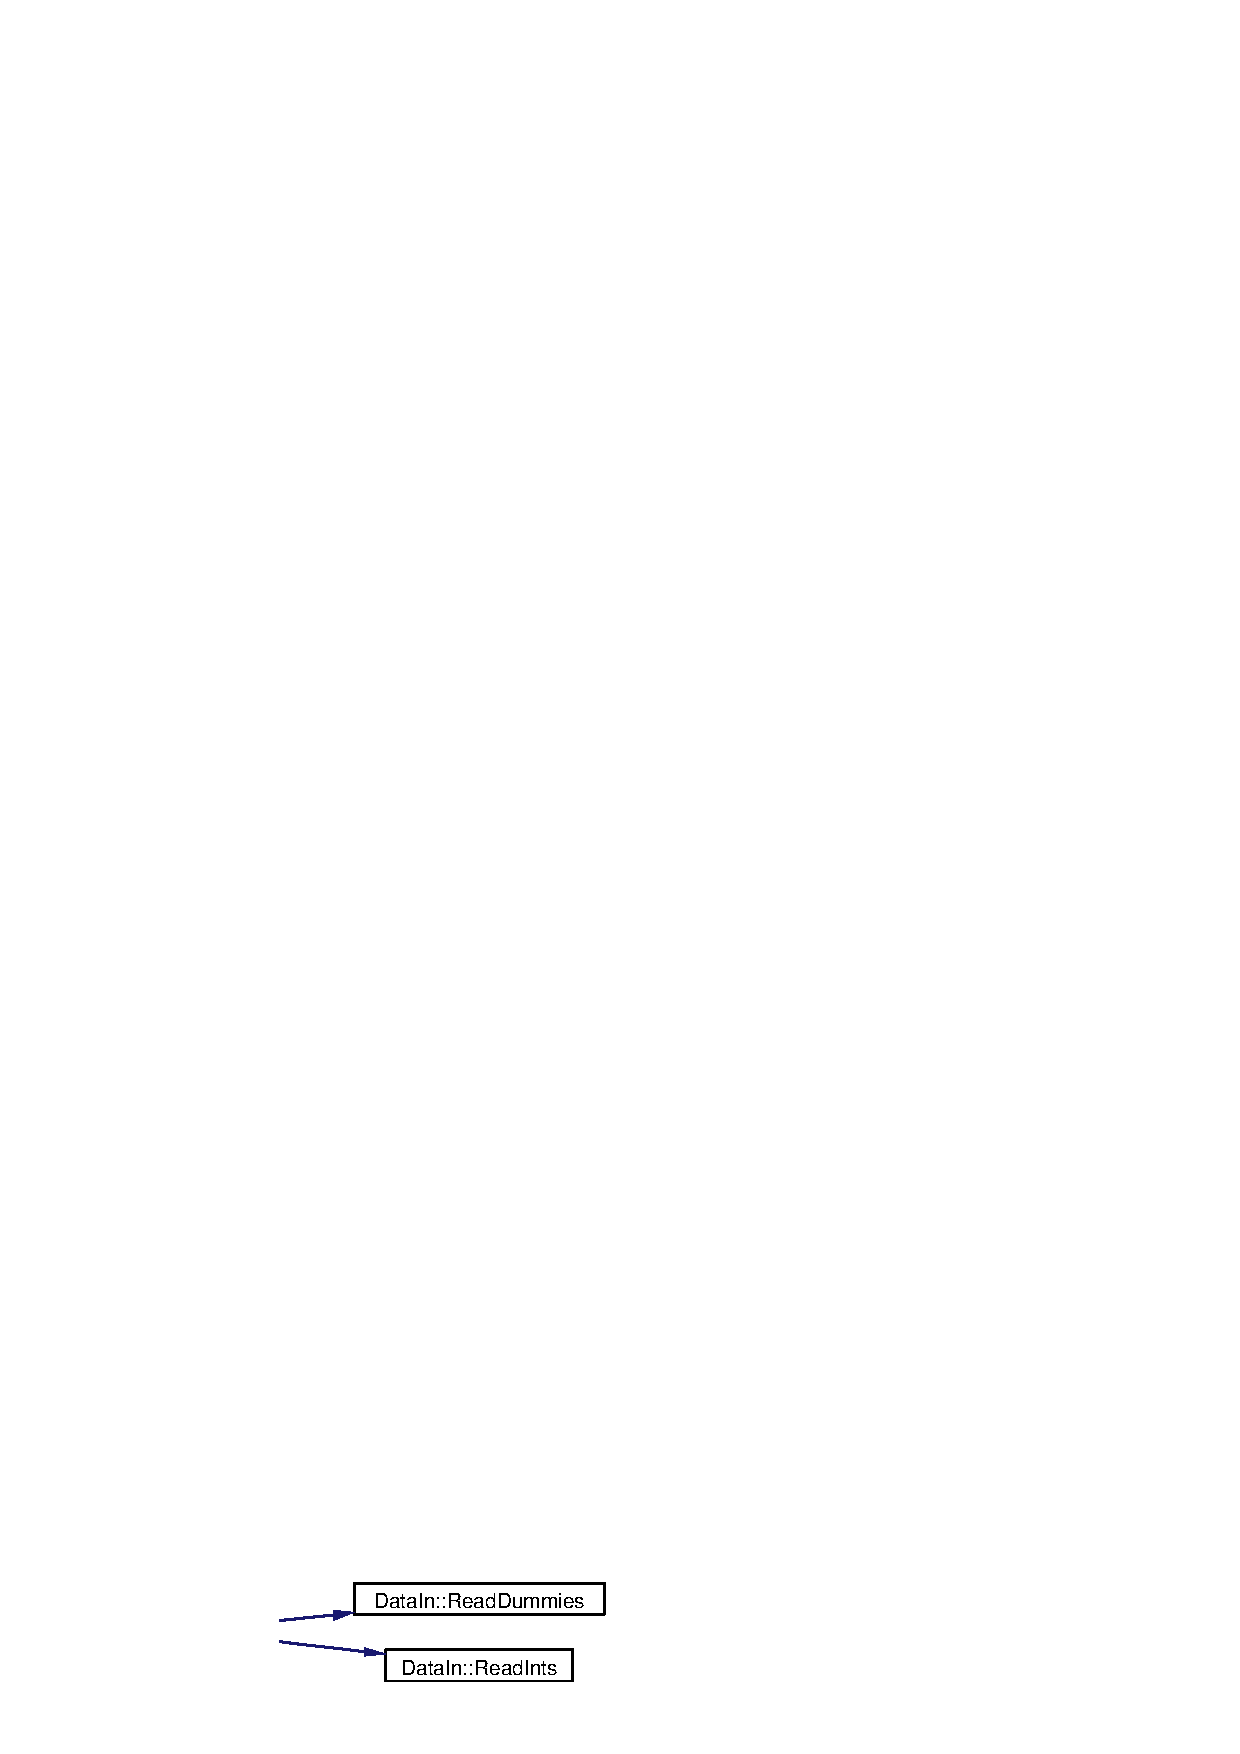
\includegraphics[width=149pt]{classEvent_a24_cgraph}
\end{center}
\end{figure}
\index{Event@{Event}!NewAttackMethods@{NewAttackMethods}}
\index{NewAttackMethods@{NewAttackMethods}!Event@{Event}}
\subsubsection{\setlength{\rightskip}{0pt plus 5cm}void Event::New\-Attack\-Methods ({\bf File\-Value} {\em args})}\label{classEvent_a34}


Choosing a method to determine attack times \begin{Desc}
\item[Parameters:]
\begin{description}
\item[{\em args}]{\bf File\-Value}{\rm (p.\,\pageref{classFileValue})} of attack methods to use \end{description}
\end{Desc}


Definition at line 683 of file event.cpp.

References Attacks(), File\-Value::get\-List\-Ptr(), and sever.

Referenced by Build\-Sub\-Events().

Here is the call graph for this function:\begin{figure}[H]
\begin{center}
\leavevmode
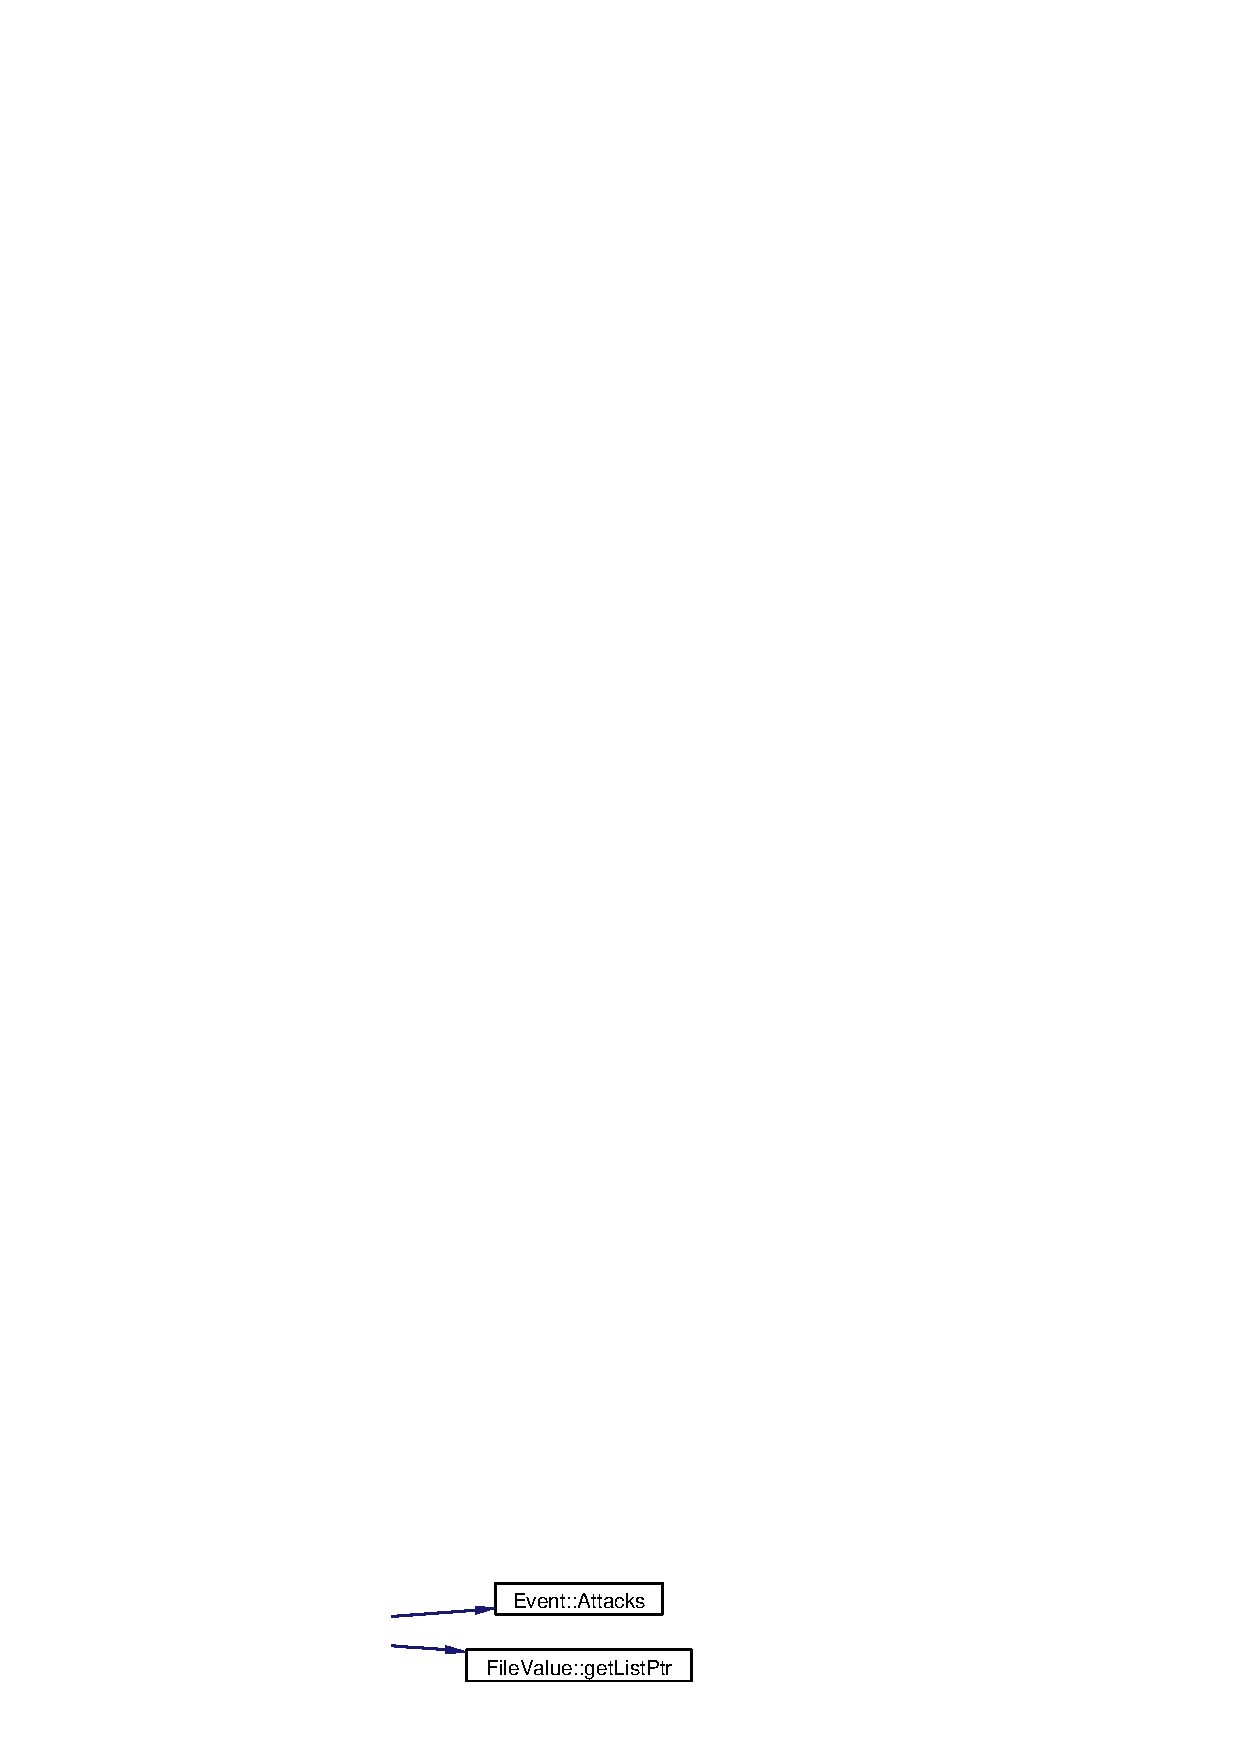
\includegraphics[width=170pt]{classEvent_a34_cgraph}
\end{center}
\end{figure}
\index{Event@{Event}!NewCopyName@{NewCopyName}}
\index{NewCopyName@{NewCopyName}!Event@{Event}}
\subsubsection{\setlength{\rightskip}{0pt plus 5cm}void Event::New\-Copy\-Name (list$<$ {\bf File\-Value} $>$ {\em data})}\label{classEvent_a29}


Reads the names of the files defining the elements of the next level and stores them in the two dimenssional character array Name\-Type. 

Definition at line 634 of file event.cpp.

References max\-Types, and name\-Type.

Referenced by Build().\index{Event@{Event}!NewCreateMatrices@{NewCreateMatrices}}
\index{NewCreateMatrices@{NewCreateMatrices}!Event@{Event}}
\subsubsection{\setlength{\rightskip}{0pt plus 5cm}void Event::New\-Create\-Matrices ({\bf File\-Value} {\em args})}\label{classEvent_a51}


First creates a \char`\"{}generic matrix\char`\"{} of attacks (or units or max sieve elements) $\ast$ obj types. It will be modified as choices are made. Then, a second matrix of durations (in matrix units) $\ast$ obj\_\-types is created . \begin{Desc}
\item[Parameters:]
\begin{description}
\item[{\em args}]{\bf File\-Value}{\rm (p.\,\pageref{classFileValue})} with a matrix vector and two lists of envelopes \end{description}
\end{Desc}


Definition at line 1039 of file event.cpp.

References array\-Size, d0, dur\-Len, Matrix::Envelopes(), File\-Value::Evaluate(), File\-Value::get\-List(), File\-Value::get\-List\-Ptr(), Matrix::Get\-Vector(), Matrix::Include\-Array(), list\-Len, Matrix, max\-Types, prob\-Sieve\-Array, and s0.

Referenced by Build\-Sub\-Events().

Here is the call graph for this function:\begin{figure}[H]
\begin{center}
\leavevmode
\includegraphics[width=400pt]{classEvent_a51_cgraph}
\end{center}
\end{figure}
\index{Event@{Event}!NewDurationMethods@{NewDurationMethods}}
\index{NewDurationMethods@{NewDurationMethods}!Event@{Event}}
\subsubsection{\setlength{\rightskip}{0pt plus 5cm}void Event::New\-Duration\-Methods ({\bf File\-Value} {\em args})}\label{classEvent_a36}


Choosing a method to determine durations. /param args A {\bf File\-Value}{\rm (p.\,\pageref{classFileValue})} of the duration methods to use 

Definition at line 786 of file event.cpp.

References File\-Value::get\-List(), Points\-Probs(), and sever.

Referenced by Build\-Sub\-Events().

Here is the call graph for this function:\begin{figure}[H]
\begin{center}
\leavevmode
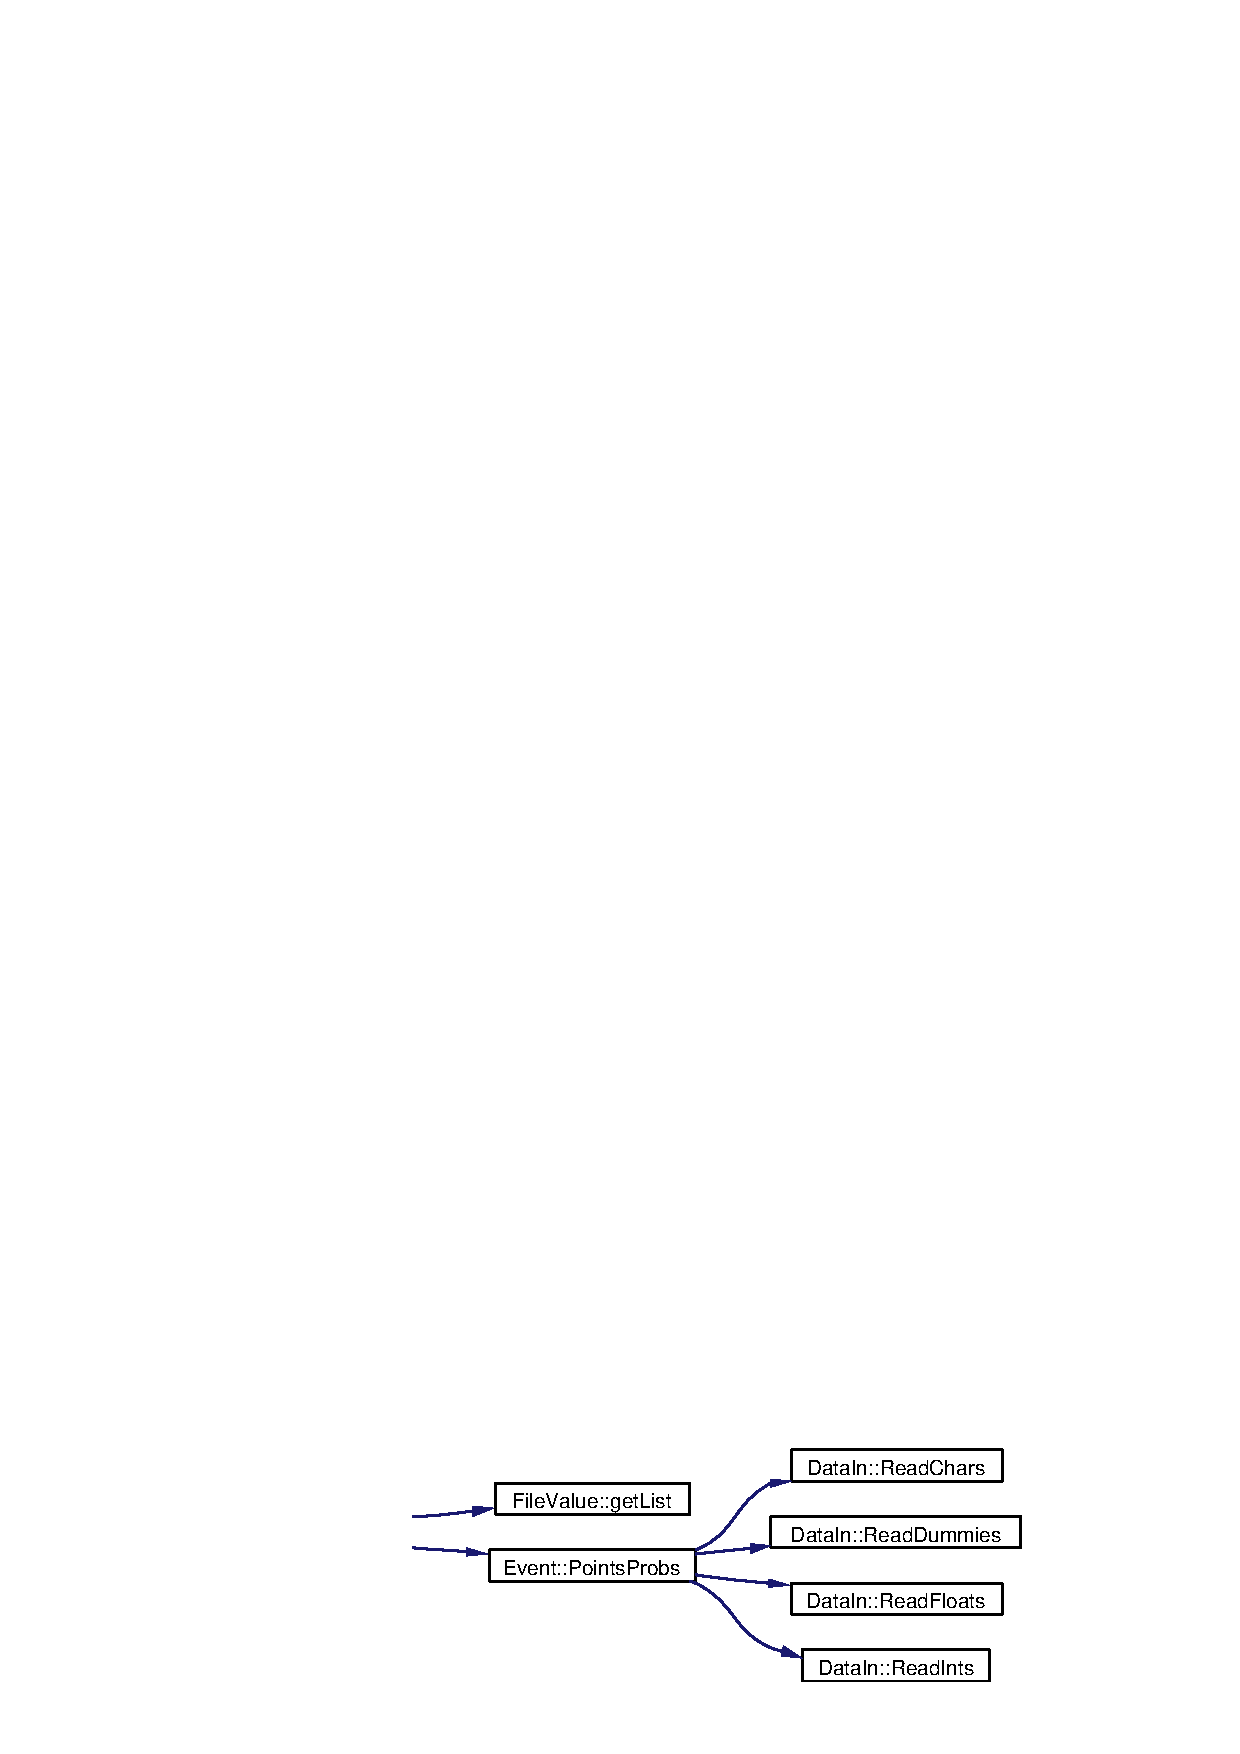
\includegraphics[width=249pt]{classEvent_a36_cgraph}
\end{center}
\end{figure}
\index{Event@{Event}!NewLayerDef@{NewLayerDef}}
\index{NewLayerDef@{NewLayerDef}!Event@{Event}}
\subsubsection{\setlength{\rightskip}{0pt plus 5cm}void Event::New\-Layer\-Def (list$<$ {\bf File\-Value} $>$ {\em data})}\label{classEvent_a25}


Determines how many layers or streams are active in this event (similar to \char`\"{}voices\char`\"{}) and how many types of objects are in each layer. 

Definition at line 444 of file event.cpp.

References bar\-Len, max\-Types, num\-Layers, obj\-Max\-Dur, types\-In\-Layer, and u\-Per\-Sec.

Referenced by Build().\index{Event@{Event}!NewNumObjs@{NewNumObjs}}
\index{NewNumObjs@{NewNumObjs}!Event@{Event}}
\subsubsection{\setlength{\rightskip}{0pt plus 5cm}void Event::New\-Num\-Objs (list$<$ {\bf File\-Value} $>$ {\em data})}\label{classEvent_a27}


Determines how many objects are in each layer according to a `given density per layer \begin{Desc}
\item[Parameters:]
\begin{description}
\item[{\em data}]File\-Values to pass in for new objects \end{description}
\end{Desc}


Definition at line 541 of file event.cpp.

References layer\-Dens, num\-Layers, num\-Objs, objs\-In\-Layer, remain\-Objs, sever, Sounds\-Per\-Sec(), and the\-Duration.

Referenced by Event\-Factory::Build(), and Build().

Here is the call graph for this function:\begin{figure}[H]
\begin{center}
\leavevmode
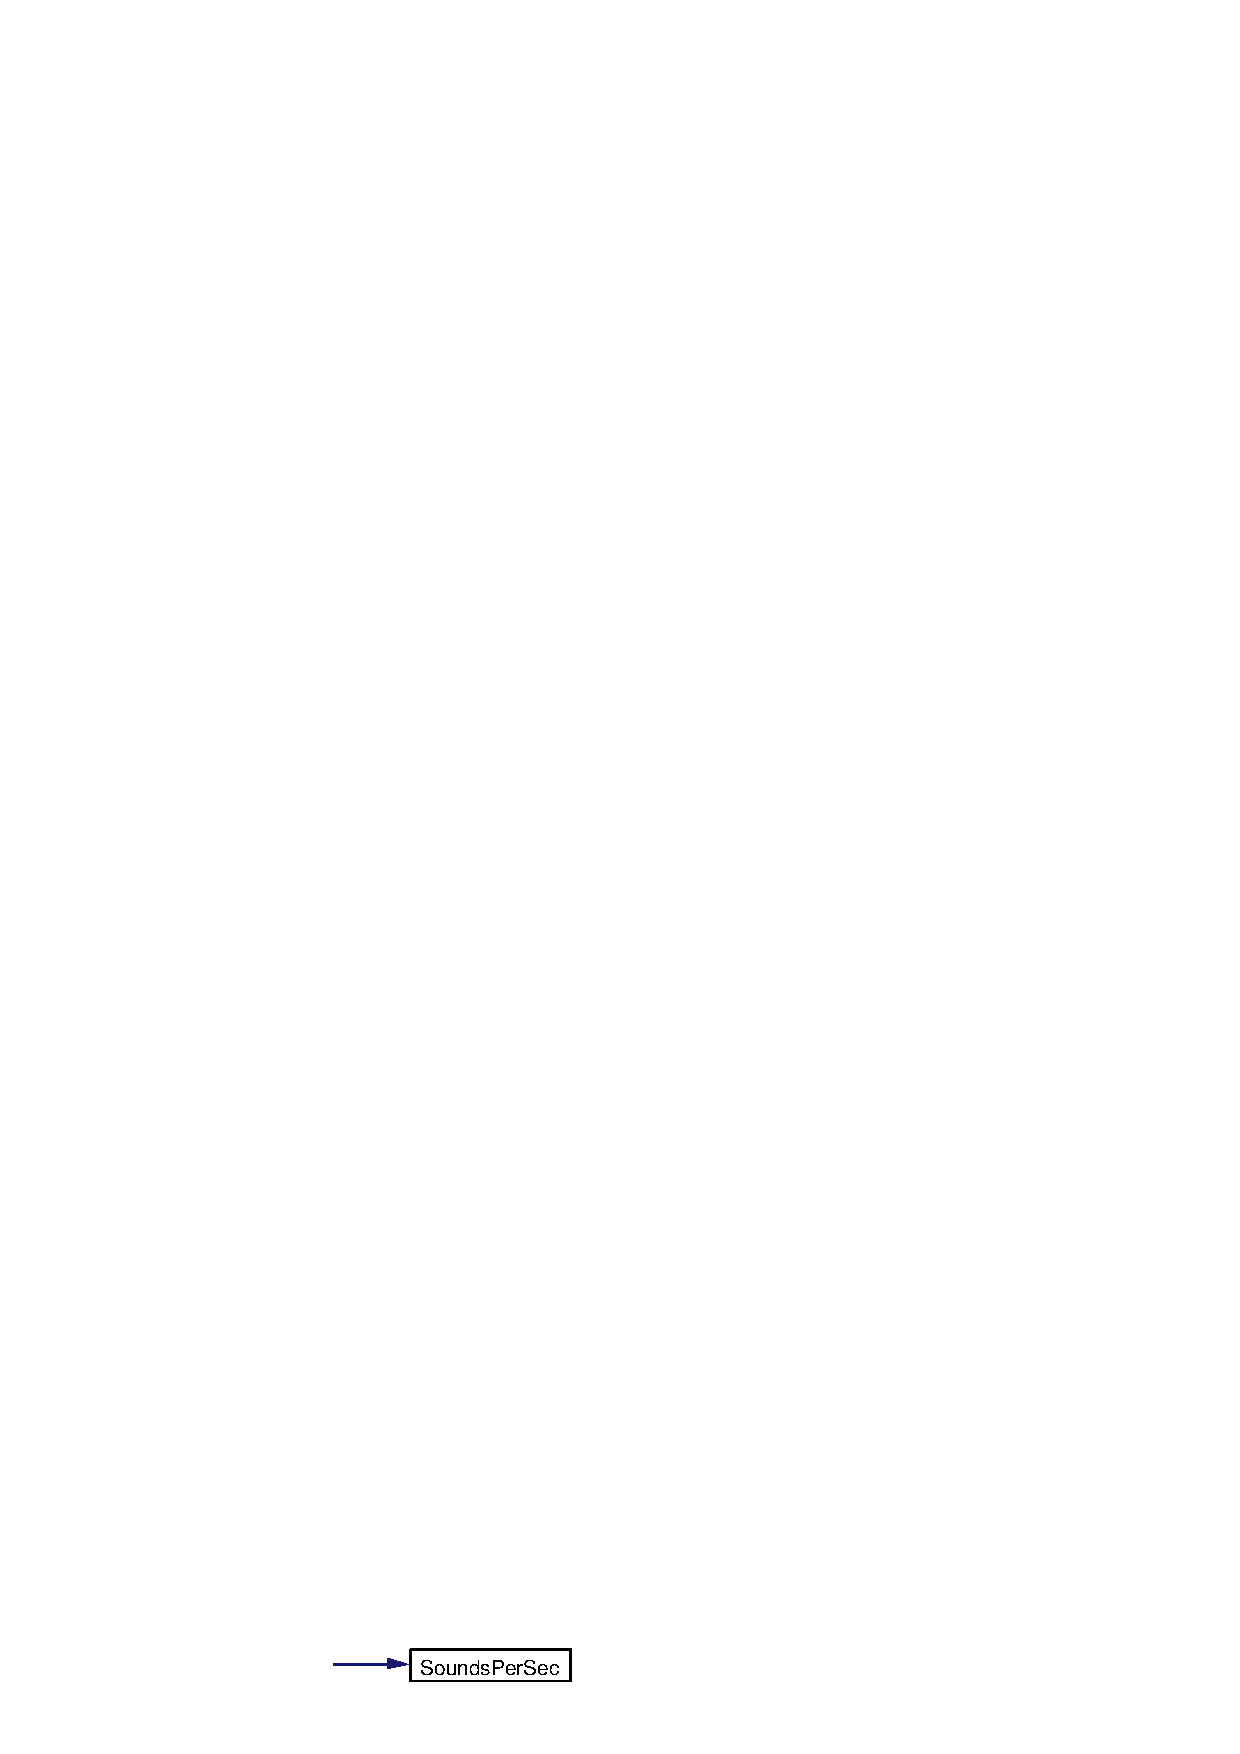
\includegraphics[width=141pt]{classEvent_a27_cgraph}
\end{center}
\end{figure}
\index{Event@{Event}!NumObjs@{NumObjs}}
\index{NumObjs@{NumObjs}!Event@{Event}}
\subsubsection{\setlength{\rightskip}{0pt plus 5cm}void Event::Num\-Objs ()}\label{classEvent_a26}


Determines how many objects are in each layer according to a `given density per layer 

\begin{Desc}
\item[{\bf Deprecated}]Use {\bf New\-Num\-Objs()}{\rm (p.\,\pageref{classEvent_a27})} instead \end{Desc}


Definition at line 485 of file event.cpp.

References check\-Point, Choose\-Offset(), Data\-In::file\-Loc(), layer\-Dens, Data\-In::name\-Of, num\-Layers, num\-Objs, objs\-In\-Layer, Data\-In::Read\-Chars(), Read\-Compute\-Float(), Read\-Compute\-Int(), Data\-In::Read\-Dummies(), remain\-Objs, Data\-In::rewind\-File(), sever, Sounds\-Per\-Sec(), and the\-Duration.

Here is the call graph for this function:\begin{figure}[H]
\begin{center}
\leavevmode
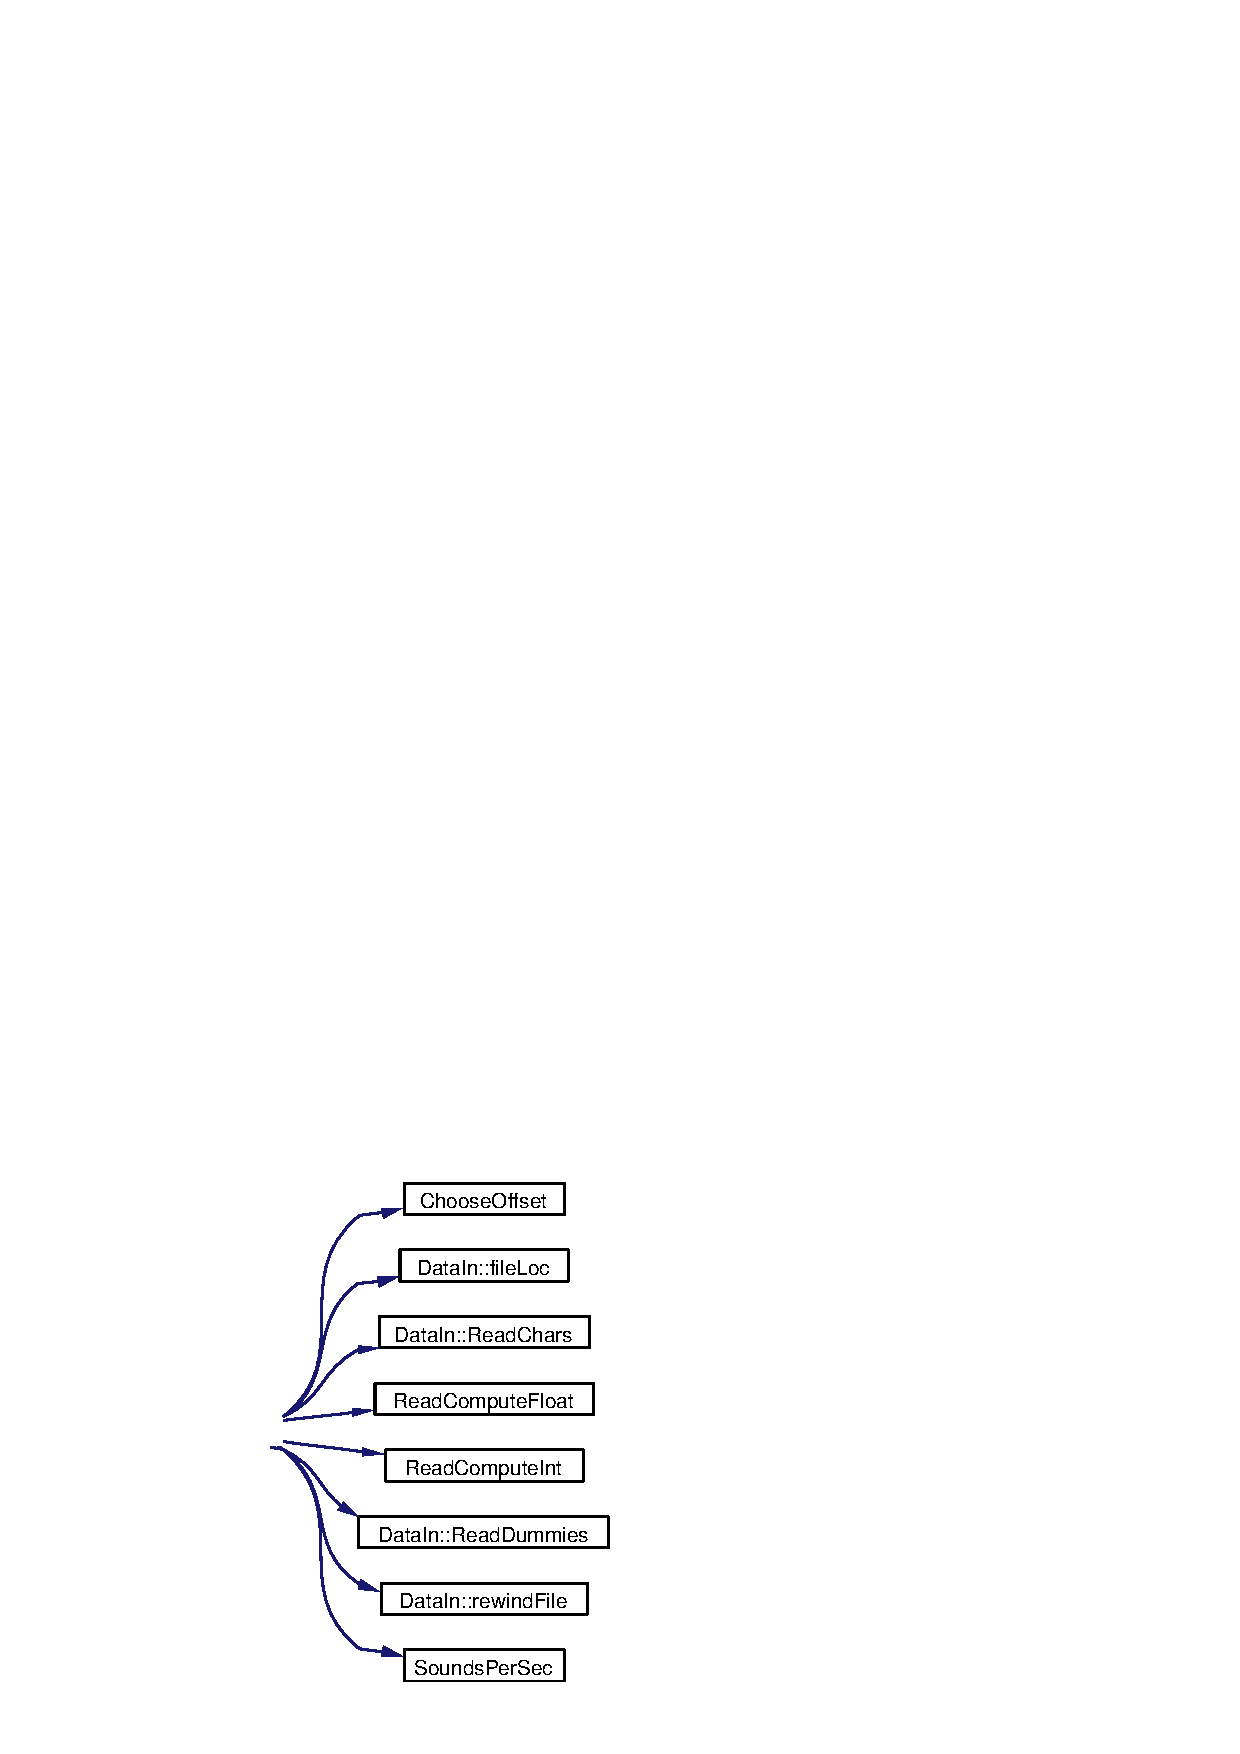
\includegraphics[width=150pt]{classEvent_a26_cgraph}
\end{center}
\end{figure}
\index{Event@{Event}!ObjCoordinates@{ObjCoordinates}}
\index{ObjCoordinates@{ObjCoordinates}!Event@{Event}}
\subsubsection{\setlength{\rightskip}{0pt plus 5cm}void Event::Obj\-Coordinates ()}\label{classEvent_a52}


Copy the original matrix, include the sieve weights and choose an attack (expressed as location in the sieve) and a obj type. 

Definition at line 1114 of file event.cpp.

References Matrix::Choose\-M(), Matrix::col, Matrix::Include\-Array(), Matrix, max\-Types, Matrix::Print(), Matrix::Print\-Vector(), Matrix::row, s0, s1, stime\-Matrix, and type.

Referenced by Discrete3().

Here is the call graph for this function:\begin{figure}[H]
\begin{center}
\leavevmode
\includegraphics[width=221pt]{classEvent_a52_cgraph}
\end{center}
\end{figure}
\index{Event@{Event}!operator=@{operator=}}
\index{operator=@{operator=}!Event@{Event}}
\subsubsection{\setlength{\rightskip}{0pt plus 5cm}{\bf Event} \& Event::operator= (const {\bf Event} \& {\em orig\-Event})}\label{classEvent_a6}


This assigns one Event to another. \begin{Desc}
\item[Parameters:]
\begin{description}
\item[{\em orig\-Event}]The Event to assign \end{description}
\end{Desc}


Definition at line 178 of file event.cpp.

References the\-Duration, the\-Name, and the\-Start\-Time.\index{Event@{Event}!Parameters@{Parameters}}
\index{Parameters@{Parameters}!Event@{Event}}
\subsubsection{\setlength{\rightskip}{0pt plus 5cm}void Event::Parameters (int {\em other\-Params})}\label{classEvent_a46}


Handles all parameters besides stime, type, and duration. could control ranges (duration, freq. register, modifiers [scales ?] -\begin{itemize}
\item like filters or masks or sieves? -, densities, and contrast between objects. \end{itemize}


\begin{Desc}
\item[{\bf Deprecated}]DO NOT USE \end{Desc}


Definition at line 1890 of file event.cpp.\index{Event@{Event}!PointsProbs@{PointsProbs}}
\index{PointsProbs@{PointsProbs}!Event@{Event}}
\subsubsection{\setlength{\rightskip}{0pt plus 5cm}void Event::Points\-Probs (const char $\ast$ {\em e\-Method}, vector$<$ int $>$ {\em e\-Arg\-Vector}, const char $\ast$ {\em w\-Method}, vector$<$ int $>$ {\em w\-Arg\-Vector})}\label{classEvent_a40}


Reads in two arrays at a time according to the method desired: for POINTS, one with all possible attacks (star\-Tarray/stimes\-Matrix) and one with their probabilities; for INTERVALS, one with all possible durations and a second with their probabilities. \begin{Desc}
\item[Parameters:]
\begin{description}
\item[{\em e\-Method}]e-Method for {\bf Sieve}{\rm (p.\,\pageref{classSieve})} \item[{\em e\-Arg\-Vector}]e-Vector for {\bf Sieve}{\rm (p.\,\pageref{classSieve})} \item[{\em w\-Method}]w-Method for {\bf Sieve}{\rm (p.\,\pageref{classSieve})} \item[{\em w\-Arg\-Vector}]w-Vector for {\bf Sieve}{\rm (p.\,\pageref{classSieve})} \end{description}
\end{Desc}


Definition at line 983 of file event.cpp.

References array\-Size, Sieve::Build(), dur\-Array, dur\-Len, Sieve::Fill\-In\-Arrays(), Sieve::Get\-List\-Len(), list\-Len, prob\-Dur\-Array, the\-Duration, and u\-Per\-Sec.

Here is the call graph for this function:\begin{figure}[H]
\begin{center}
\leavevmode
\includegraphics[width=301pt]{classEvent_a40_cgraph}
\end{center}
\end{figure}
\index{Event@{Event}!PointsProbs@{PointsProbs}}
\index{PointsProbs@{PointsProbs}!Event@{Event}}
\subsubsection{\setlength{\rightskip}{0pt plus 5cm}void Event::Points\-Probs ()}\label{classEvent_a39}


Reads in two arrays at a time according to the method desired: for POINTS, one with all possible attacks (star\-Tarray/stimes\-Matrix) and one with their probabilities; for INTERVALS, one with all possible durations and a second with their probabilities. 

\begin{Desc}
\item[{\bf Deprecated}]DO NOT USE (use Points\-Probs(char$\ast$, vector$<$int$>$, char$\ast$, vector$<$int$>$) instead) \end{Desc}


Definition at line 923 of file event.cpp.

References dur\-Array, dur\-Len, Data\-In::float\-Vect, Data\-In::int\-Vect, list\-Len, Data\-In::name\-Of, prob\-Dur\-Array, prob\-Sieve\-Array, Data\-In::Read\-Chars(), Data\-In::Read\-Dummies(), Data\-In::Read\-Floats(), Data\-In::Read\-Ints(), sever, and star\-Tarray.

Referenced by Duration\-Methods(), and New\-Duration\-Methods().

Here is the call graph for this function:\begin{figure}[H]
\begin{center}
\leavevmode
\includegraphics[width=154pt]{classEvent_a39_cgraph}
\end{center}
\end{figure}
\index{Event@{Event}!Print@{Print}}
\index{Print@{Print}!Event@{Event}}
\subsubsection{\setlength{\rightskip}{0pt plus 5cm}void Event::Print ()\hspace{0.3cm}{\tt  [virtual]}}\label{classEvent_a57}




Reimplemented in {\bf Bottom} {\rm (p.\,\pageref{classBottom_a30})}, {\bf High} {\rm (p.\,\pageref{classHigh_a5})}, {\bf Low} {\rm (p.\,\pageref{classLow_a5})}, and {\bf Top} {\rm (p.\,\pageref{classTop_a8})}.

Definition at line 2046 of file event.cpp.

References name\-Type, num\-Objs, subevents, the\-Duration, the\-Name, the\-Start\-Time, and the\-Type.

Referenced by Event\-Factory::Build(), and build\-Note().\index{Event@{Event}!SelectNextEvent@{SelectNextEvent}}
\index{SelectNextEvent@{SelectNextEvent}!Event@{Event}}
\subsubsection{\setlength{\rightskip}{0pt plus 5cm}void Event::Select\-Next\-Event ()}\label{classEvent_a45}


Identifies the type of the next object, calls its constructor and opens the file associated with it. Then, it calls Build and Create\-New\-Objects in a recursive process. 

\begin{Desc}
\item[{\bf Deprecated}]NOT IMPLEMENTED - DO NOT USE \end{Desc}
\index{Event@{Event}!setBottomFreq@{setBottomFreq}}
\index{setBottomFreq@{setBottomFreq}!Event@{Event}}
\subsubsection{\setlength{\rightskip}{0pt plus 5cm}void Event::set\-Bottom\-Freq ({\bf File\-Value} $\ast$ {\em s})\hspace{0.3cm}{\tt  [inline]}}\label{classEvent_a61}


Set bottom frequency \begin{Desc}
\item[Parameters:]
\begin{description}
\item[{\em s}]A {\bf File\-Value}{\rm (p.\,\pageref{classFileValue})} $\ast$ to the new bottom frequency of the event \end{description}
\end{Desc}


Definition at line 546 of file event.h.

References bottom\_\-frequency.

Referenced by Event\-Factory::Build().\index{Event@{Event}!setBottomLoud@{setBottomLoud}}
\index{setBottomLoud@{setBottomLoud}!Event@{Event}}
\subsubsection{\setlength{\rightskip}{0pt plus 5cm}void Event::set\-Bottom\-Loud ({\bf File\-Value} $\ast$ {\em s})\hspace{0.3cm}{\tt  [inline]}}\label{classEvent_a63}


Set bottom loudness \begin{Desc}
\item[Parameters:]
\begin{description}
\item[{\em s}]A {\bf File\-Value}{\rm (p.\,\pageref{classFileValue})} $\ast$ to the new bottom loudness of the event \end{description}
\end{Desc}


Definition at line 557 of file event.h.

References bottom\_\-loudness.

Referenced by Event\-Factory::Build().\index{Event@{Event}!setDensity@{setDensity}}
\index{setDensity@{setDensity}!Event@{Event}}
\subsubsection{\setlength{\rightskip}{0pt plus 5cm}void Event::set\-Density (double {\em a\-Density})\hspace{0.3cm}{\tt  [virtual]}}\label{classEvent_a11}


Sets the density of the event \begin{Desc}
\item[Parameters:]
\begin{description}
\item[{\em a\-Density}]Density of the event \end{description}
\end{Desc}


Reimplemented in {\bf Bottom} {\rm (p.\,\pageref{classBottom_a9})}.

Definition at line 269 of file event.cpp.

References the\-Density.

Referenced by High::High(), and Low::Low().\index{Event@{Event}!setDuration@{setDuration}}
\index{setDuration@{setDuration}!Event@{Event}}
\subsubsection{\setlength{\rightskip}{0pt plus 5cm}void Event::set\-Duration (float {\em a\-Duration})\hspace{0.3cm}{\tt  [virtual]}}\label{classEvent_a8}


Sets the duration of the event \begin{Desc}
\item[Parameters:]
\begin{description}
\item[{\em a\-Duration}]Duration of the event \end{description}
\end{Desc}


Reimplemented in {\bf Bottom} {\rm (p.\,\pageref{classBottom_a8})}.

Definition at line 242 of file event.cpp.

References the\-Duration.

Referenced by Event(), High::High(), Low::Low(), and Top::Top().\index{Event@{Event}!setName@{setName}}
\index{setName@{setName}!Event@{Event}}
\subsubsection{\setlength{\rightskip}{0pt plus 5cm}void Event::set\-Name (char $\ast$ {\em a\-Name})\hspace{0.3cm}{\tt  [virtual]}}\label{classEvent_a10}


Sets the name of the event \begin{Desc}
\item[Parameters:]
\begin{description}
\item[{\em a\-Name}]Name of the event \end{description}
\end{Desc}


Reimplemented in {\bf Bottom} {\rm (p.\,\pageref{classBottom_a6})}.

Definition at line 252 of file event.cpp.

References the\-Name.

Referenced by Event(), High::High(), Low::Low(), and Top::Top().\index{Event@{Event}!setNoteDynamicMark@{setNoteDynamicMark}}
\index{setNoteDynamicMark@{setNoteDynamicMark}!Event@{Event}}
\subsubsection{\setlength{\rightskip}{0pt plus 5cm}void Event::set\-Note\-Dynamic\-Mark ({\bf File\-Value} $\ast$ {\em s})\hspace{0.3cm}{\tt  [inline]}}\label{classEvent_a79}


Set note\_\-dynamic\-Mark for event \begin{Desc}
\item[Parameters:]
\begin{description}
\item[{\em s}]A {\bf File\-Value}{\rm (p.\,\pageref{classFileValue})} $\ast$ to new note\_\-dynamic\-Mark for the event \end{description}
\end{Desc}


Definition at line 645 of file event.h.

References note\_\-dynamic\-Mark.

Referenced by Event\-Factory::Build().\index{Event@{Event}!setNoteModifiers@{setNoteModifiers}}
\index{setNoteModifiers@{setNoteModifiers}!Event@{Event}}
\subsubsection{\setlength{\rightskip}{0pt plus 5cm}void Event::set\-Note\-Modifiers ({\bf File\-Value} $\ast$ {\em s})\hspace{0.3cm}{\tt  [inline]}}\label{classEvent_a81}


Set note\_\-modifiers for event \begin{Desc}
\item[Parameters:]
\begin{description}
\item[{\em s}]A {\bf File\-Value}{\rm (p.\,\pageref{classFileValue})} $\ast$ to new note\_\-modifiers for the event \end{description}
\end{Desc}


Definition at line 656 of file event.h.

References note\_\-modifiers.

Referenced by Event\-Factory::Build().\index{Event@{Event}!setNotePitchClass@{setNotePitchClass}}
\index{setNotePitchClass@{setNotePitchClass}!Event@{Event}}
\subsubsection{\setlength{\rightskip}{0pt plus 5cm}void Event::set\-Note\-Pitch\-Class ({\bf File\-Value} $\ast$ {\em s})\hspace{0.3cm}{\tt  [inline]}}\label{classEvent_a77}


Set note\_\-pitch\-Class for event \begin{Desc}
\item[Parameters:]
\begin{description}
\item[{\em s}]A {\bf File\-Value}{\rm (p.\,\pageref{classFileValue})} $\ast$ to new note\_\-pitch\-Class for the event \end{description}
\end{Desc}


Definition at line 634 of file event.h.

References note\_\-pitch\-Class.

Referenced by Event\-Factory::Build().\index{Event@{Event}!setSoundDeviation@{setSoundDeviation}}
\index{setSoundDeviation@{setSoundDeviation}!Event@{Event}}
\subsubsection{\setlength{\rightskip}{0pt plus 5cm}void Event::set\-Sound\-Deviation ({\bf File\-Value} $\ast$ {\em s})\hspace{0.3cm}{\tt  [inline]}}\label{classEvent_a67}


Set sound\_\-deviation for event \begin{Desc}
\item[Parameters:]
\begin{description}
\item[{\em s}]A {\bf File\-Value}{\rm (p.\,\pageref{classFileValue})} $\ast$ to new sound\_\-deviation for the event \end{description}
\end{Desc}


Definition at line 579 of file event.h.

References sound\_\-deviation.

Referenced by Event\-Factory::Build().\index{Event@{Event}!setSoundModifiers@{setSoundModifiers}}
\index{setSoundModifiers@{setSoundModifiers}!Event@{Event}}
\subsubsection{\setlength{\rightskip}{0pt plus 5cm}void Event::set\-Sound\-Modifiers ({\bf File\-Value} $\ast$ {\em s})\hspace{0.3cm}{\tt  [inline]}}\label{classEvent_a71}


Set sound\_\-modifiers for event /param s A {\bf File\-Value}{\rm (p.\,\pageref{classFileValue})} $\ast$ to new sound\_\-modifiers for the event 

Definition at line 601 of file event.h.

References sound\_\-modifiers.

Referenced by Event\-Factory::Build().\index{Event@{Event}!setSoundNumPartials@{setSoundNumPartials}}
\index{setSoundNumPartials@{setSoundNumPartials}!Event@{Event}}
\subsubsection{\setlength{\rightskip}{0pt plus 5cm}void Event::set\-Sound\-Num\-Partials ({\bf File\-Value} $\ast$ {\em s})\hspace{0.3cm}{\tt  [inline]}}\label{classEvent_a65}


Set sound\_\-num\-Partials for event \begin{Desc}
\item[Parameters:]
\begin{description}
\item[{\em s}]A {\bf File\-Value}{\rm (p.\,\pageref{classFileValue})} $\ast$ to new sound\_\-num\-Partials for the event \end{description}
\end{Desc}


Definition at line 568 of file event.h.

References sound\_\-num\-Partials.

Referenced by Event\-Factory::Build().\index{Event@{Event}!setSoundPartEnvs@{setSoundPartEnvs}}
\index{setSoundPartEnvs@{setSoundPartEnvs}!Event@{Event}}
\subsubsection{\setlength{\rightskip}{0pt plus 5cm}void Event::set\-Sound\-Part\-Envs ({\bf File\-Value} $\ast$ {\em s})\hspace{0.3cm}{\tt  [inline]}}\label{classEvent_a69}


Set sound\_\-part\-Envs for event \begin{Desc}
\item[Parameters:]
\begin{description}
\item[{\em s}]A {\bf File\-Value}{\rm (p.\,\pageref{classFileValue})} $\ast$ to new sound\_\-part\-Envs for the event \end{description}
\end{Desc}


Definition at line 590 of file event.h.

References sound\_\-part\-Envs.

Referenced by Event\-Factory::Build().\index{Event@{Event}!setSoundReverberation@{setSoundReverberation}}
\index{setSoundReverberation@{setSoundReverberation}!Event@{Event}}
\subsubsection{\setlength{\rightskip}{0pt plus 5cm}void Event::set\-Sound\-Reverberation ({\bf File\-Value} $\ast$ {\em s})\hspace{0.3cm}{\tt  [inline]}}\label{classEvent_a73}


Set sound\_\-reverberation for event \begin{Desc}
\item[Parameters:]
\begin{description}
\item[{\em s}]A {\bf File\-Value}{\rm (p.\,\pageref{classFileValue})} $\ast$ to new sound\_\-reverberation for the event \end{description}
\end{Desc}


Definition at line 612 of file event.h.

References sound\_\-reverberation.\index{Event@{Event}!setSoundSpatialization@{setSoundSpatialization}}
\index{setSoundSpatialization@{setSoundSpatialization}!Event@{Event}}
\subsubsection{\setlength{\rightskip}{0pt plus 5cm}void Event::set\-Sound\-Spatialization ({\bf File\-Value} $\ast$ {\em s})\hspace{0.3cm}{\tt  [inline]}}\label{classEvent_a75}


Set sound\_\-spatialization for event \begin{Desc}
\item[Parameters:]
\begin{description}
\item[{\em s}]A {\bf File\-Value}{\rm (p.\,\pageref{classFileValue})} $\ast$ to new sound\_\-spatialization for the event \end{description}
\end{Desc}


Definition at line 623 of file event.h.

References sound\_\-spatialization.\index{Event@{Event}!setStartDurationType@{setStartDurationType}}
\index{setStartDurationType@{setStartDurationType}!Event@{Event}}
\subsubsection{\setlength{\rightskip}{0pt plus 5cm}void Event::set\-Start\-Duration\-Type (list$<$ {\bf File\-Value} $>$ {\em data})}\label{classEvent_a47}


\begin{Desc}
\item[{\bf Deprecated}]DO NOT USE \end{Desc}
\index{Event@{Event}!setStartTime@{setStartTime}}
\index{setStartTime@{setStartTime}!Event@{Event}}
\subsubsection{\setlength{\rightskip}{0pt plus 5cm}void Event::set\-Start\-Time (float {\em a\-Start\-Time})\hspace{0.3cm}{\tt  [virtual]}}\label{classEvent_a7}


Sets the start time of the event \begin{Desc}
\item[Parameters:]
\begin{description}
\item[{\em a\-Start\-Time}]Start time for the event \end{description}
\end{Desc}


Reimplemented in {\bf Bottom} {\rm (p.\,\pageref{classBottom_a7})}, and {\bf Top} {\rm (p.\,\pageref{classTop_a5})}.

Definition at line 209 of file event.cpp.

References the\-Start\-Time.

Referenced by Event(), High::High(), and Low::Low().\index{Event@{Event}!setType@{setType}}
\index{setType@{setType}!Event@{Event}}
\subsubsection{\setlength{\rightskip}{0pt plus 5cm}void Event::set\-Type (int {\em a\-Type})\hspace{0.3cm}{\tt  [virtual]}}\label{classEvent_a9}


Sets the type of the event \begin{Desc}
\item[Parameters:]
\begin{description}
\item[{\em a\-Type}]Type of the event \end{description}
\end{Desc}


Definition at line 224 of file event.cpp.

References the\-Type.

Referenced by Event(), High::High(), and Low::Low().\index{Event@{Event}!Stimes@{Stimes}}
\index{Stimes@{Stimes}!Event@{Event}}
\subsubsection{\setlength{\rightskip}{0pt plus 5cm}int Event::Stimes ()}\label{classEvent_a42}


\begin{Desc}
\item[{\bf Deprecated}]DO NOT USE (Used to be private... not sure why it isn't anymore) \end{Desc}


Reimplemented in {\bf Top} {\rm (p.\,\pageref{classTop_d0})}.

Definition at line 1350 of file event.cpp.

References array\-Size, GSection(), List$<$ Etype $>$::Head(), List$<$ Etype $>$::Insert\-In\-Order(), Data\-In::int\-Vect, List$<$ Etype $>$::Length(), levels, Data\-In::Read\-Ints(), List$<$ Etype $>$::Retrieve(), star\-Tarray, the\-Duration, and u\-Per\-Sec.

Here is the call graph for this function:\begin{figure}[H]
\begin{center}
\leavevmode
\includegraphics[width=257pt]{classEvent_a42_cgraph}
\end{center}
\end{figure}
\index{Event@{Event}!Sweep3@{Sweep3}}
\index{Sweep3@{Sweep3}!Event@{Event}}
\subsubsection{\setlength{\rightskip}{0pt plus 5cm}void Event::Sweep3 ()}\label{classEvent_a32}


DEPRECATED

Sweep3. Method for assigning stime\-Sec and dur\-Sec values in sequential order - \char`\"{}sweepeing\char`\"{} from left to right or beginning to end of the event. For stime and duration two different methods are used, one for integer values the other for float values. Type being a discrete value, the integer values method is used for it. 

Definition at line 1766 of file event.cpp.

References check\-Point, Choose\-Offset(), dur\-Sec, lastime, Data\-In::name\-Of, new\-Obj, obj\-Max\-Dur, Data\-In::Read\-Chars(), Read\-Compute\-Float(), Read\-Compute\-Int(), sever, stime\-Sec, the\-Duration, type, u\-Per\-Sec, and Value\-Pick().

Here is the call graph for this function:\begin{figure}[H]
\begin{center}
\leavevmode
\includegraphics[width=137pt]{classEvent_a32_cgraph}
\end{center}
\end{figure}
\index{Event@{Event}!TestNameType@{TestNameType}}
\index{TestNameType@{TestNameType}!Event@{Event}}
\subsubsection{\setlength{\rightskip}{0pt plus 5cm}void Event::Test\-Name\-Type ()}\label{classEvent_a49}


Prints the test name type to standard output (cout). 

Definition at line 2006 of file event.cpp.

References max\-Types, name\-Type, num\-Chars, and sever.

Referenced by Bottom::clear().\index{Event@{Event}!TimeConvert@{TimeConvert}}
\index{TimeConvert@{TimeConvert}!Event@{Event}}
\subsubsection{\setlength{\rightskip}{0pt plus 5cm}void Event::Time\-Convert ()}\label{classEvent_a44}


Converts stime\-Matrix and dur\-Matrix as defined in the (sieve) array into time units (for notation) and into seconds (for synthesis). It also determines the check\-Point (a ) or where this object is in the larger event for use in further calculations. 

Definition at line 1323 of file event.cpp.

References check\-Point, dur\-Array, du\-Ratio, dur\-Matrix, dur\-Sec, dur\-Units, list\-Len, obj\-Max\-Dur, star\-Tarray, stime\-Matrix, stime\-Sec, stime\-Units, the\-Duration, the\-Start\-Time, and u\-Per\-Sec.

Referenced by Discrete3().

\subsection{Friends And Related Function Documentation}
\index{Event@{Event}!Matrix@{Matrix}}
\index{Matrix@{Matrix}!Event@{Event}}
\subsubsection{\setlength{\rightskip}{0pt plus 5cm}friend class {\bf Matrix}\hspace{0.3cm}{\tt  [friend]}}\label{classEvent_n0}




Definition at line 45 of file event.h.

Referenced by Find\-Dur(), New\-Create\-Matrices(), and Obj\-Coordinates().

\subsection{Member Data Documentation}
\index{Event@{Event}!aName@{aName}}
\index{aName@{aName}!Event@{Event}}
\subsubsection{\setlength{\rightskip}{0pt plus 5cm}char$\ast$ {\bf Event::a\-Name}}\label{classEvent_o9}




Definition at line 231 of file event.h.

Referenced by Bottom::Bottom(), High::High(), Low::Low(), and Top::Top().\index{Event@{Event}!arraySize@{arraySize}}
\index{arraySize@{arraySize}!Event@{Event}}
\subsubsection{\setlength{\rightskip}{0pt plus 5cm}int {\bf Event::array\-Size}}\label{classEvent_o25}




Definition at line 405 of file event.h.

Referenced by Attacks(), New\-Create\-Matrices(), Points\-Probs(), and Stimes().\index{Event@{Event}!barLen@{barLen}}
\index{barLen@{barLen}!Event@{Event}}
\subsubsection{\setlength{\rightskip}{0pt plus 5cm}int {\bf Event::bar\-Len}}\label{classEvent_o16}




Reimplemented in {\bf Note} {\rm (p.\,\pageref{classNote_r6})}.

Definition at line 400 of file event.h.

Referenced by Event\-Factory::Build(), Bottom::build\-Note(), Layer\-Def(), and New\-Layer\-Def().\index{Event@{Event}!bottom_frequency@{bottom\_\-frequency}}
\index{bottom_frequency@{bottom\_\-frequency}!Event@{Event}}
\subsubsection{\setlength{\rightskip}{0pt plus 5cm}{\bf File\-Value}$\ast$ {\bf Event::bottom\_\-frequency}\hspace{0.3cm}{\tt  [protected]}}\label{classEvent_p0}




Definition at line 519 of file event.h.

Referenced by Note::Assign\-Pitch(), get\-Bottom\-Freq(), and set\-Bottom\-Freq().\index{Event@{Event}!bottom_loudness@{bottom\_\-loudness}}
\index{bottom_loudness@{bottom\_\-loudness}!Event@{Event}}
\subsubsection{\setlength{\rightskip}{0pt plus 5cm}{\bf File\-Value}$\ast$ {\bf Event::bottom\_\-loudness}\hspace{0.3cm}{\tt  [protected]}}\label{classEvent_p1}




Definition at line 520 of file event.h.

Referenced by Note::Assign\-Loudness(), get\-Bottom\-Loud(), Bottom::Loud(), and set\-Bottom\-Loud().\index{Event@{Event}!checkPoint@{checkPoint}}
\index{checkPoint@{checkPoint}!Event@{Event}}
\subsubsection{\setlength{\rightskip}{0pt plus 5cm}double {\bf Event::check\-Point}}\label{classEvent_o0}




Definition at line 222 of file event.h.

Referenced by Event\-Factory::Build(), Bottom::build\-Note(), Bottom::build\-Sound(), Build\-Sub\-Events(), Bottom::Choose\-Sound\-Dyn\-Param(), Continuum(), Continuum3(), get\-Check\-Point(), Num\-Objs(), Bottom::Spectrum(), Sweep3(), and Time\-Convert().\index{Event@{Event}!coefParam@{coefParam}}
\index{coefParam@{coefParam}!Event@{Event}}
\subsubsection{\setlength{\rightskip}{0pt plus 5cm}float$\ast$$\ast$ {\bf Event::coef\-Param}}\label{classEvent_o52}




Definition at line 502 of file event.h.\index{Event@{Event}!d0@{d0}}
\index{d0@{d0}!Event@{Event}}
\subsubsection{\setlength{\rightskip}{0pt plus 5cm}{\bf Matrix} $\ast$ {\bf Event::d0}}\label{classEvent_o2}




Definition at line 223 of file event.h.

Referenced by Find\-Dur(), and New\-Create\-Matrices().\index{Event@{Event}!d1@{d1}}
\index{d1@{d1}!Event@{Event}}
\subsubsection{\setlength{\rightskip}{0pt plus 5cm}{\bf Matrix} $\ast$ {\bf Event::d1}}\label{classEvent_o4}




Definition at line 223 of file event.h.

Referenced by Find\-Dur().\index{Event@{Event}!dataParam@{dataParam}}
\index{dataParam@{dataParam}!Event@{Event}}
\subsubsection{\setlength{\rightskip}{0pt plus 5cm}int$\ast$$\ast$ {\bf Event::data\-Param}}\label{classEvent_o51}




Definition at line 501 of file event.h.\index{Event@{Event}!durArray@{durArray}}
\index{durArray@{durArray}!Event@{Event}}
\subsubsection{\setlength{\rightskip}{0pt plus 5cm}int$\ast$ {\bf Event::dur\-Array}}\label{classEvent_o29}




Definition at line 407 of file event.h.

Referenced by clear(), Bottom::clear(), Event(), Find\-Dur(), Find\-Len(), Points\-Probs(), and Time\-Convert().\index{Event@{Event}!duRatio@{duRatio}}
\index{duRatio@{duRatio}!Event@{Event}}
\subsubsection{\setlength{\rightskip}{0pt plus 5cm}double {\bf Event::du\-Ratio}}\label{classEvent_o41}




Definition at line 489 of file event.h.

Referenced by Time\-Convert().\index{Event@{Event}!durLen@{durLen}}
\index{durLen@{durLen}!Event@{Event}}
\subsubsection{\setlength{\rightskip}{0pt plus 5cm}int {\bf Event::dur\-Len}}\label{classEvent_o27}




Definition at line 405 of file event.h.

Referenced by Find\-Len(), New\-Create\-Matrices(), and Points\-Probs().\index{Event@{Event}!durMatrix@{durMatrix}}
\index{durMatrix@{durMatrix}!Event@{Event}}
\subsubsection{\setlength{\rightskip}{0pt plus 5cm}int {\bf Event::dur\-Matrix}}\label{classEvent_o35}




Definition at line 487 of file event.h.

Referenced by Find\-Dur(), and Time\-Convert().\index{Event@{Event}!durSec@{durSec}}
\index{durSec@{durSec}!Event@{Event}}
\subsubsection{\setlength{\rightskip}{0pt plus 5cm}float {\bf Event::dur\-Sec}}\label{classEvent_o39}




Reimplemented in {\bf Note} {\rm (p.\,\pageref{classNote_r7})}.

Definition at line 488 of file event.h.

Referenced by Bottom::build\-Note(), Bottom::build\-Sound(), Build\-Sub\-Events(), Continuum(), Continuum3(), Layer\-Def(), Bottom::Print\-Sound(), Sweep3(), and Time\-Convert().\index{Event@{Event}!durUnits@{durUnits}}
\index{durUnits@{durUnits}!Event@{Event}}
\subsubsection{\setlength{\rightskip}{0pt plus 5cm}int {\bf Event::dur\-Units}}\label{classEvent_o36}




Reimplemented in {\bf Note} {\rm (p.\,\pageref{classNote_r8})}.

Definition at line 487 of file event.h.

Referenced by Time\-Convert().\index{Event@{Event}!envParam@{envParam}}
\index{envParam@{envParam}!Event@{Event}}
\subsubsection{\setlength{\rightskip}{0pt plus 5cm}int$\ast$ {\bf Event::env\-Param}}\label{classEvent_o56}




Definition at line 507 of file event.h.\index{Event@{Event}!fname@{fname}}
\index{fname@{fname}!Event@{Event}}
\subsubsection{\setlength{\rightskip}{0pt plus 5cm}char$\ast$ {\bf Event::fname}}\label{classEvent_o48}




Definition at line 495 of file event.h.\index{Event@{Event}!keepName@{keepName}}
\index{keepName@{keepName}!Event@{Event}}
\subsubsection{\setlength{\rightskip}{0pt plus 5cm}char$\ast$ {\bf Event::keep\-Name}}\label{classEvent_o46}




Definition at line 492 of file event.h.

Referenced by Top::Top().\index{Event@{Event}!lastime@{lastime}}
\index{lastime@{lastime}!Event@{Event}}
\subsubsection{\setlength{\rightskip}{0pt plus 5cm}float {\bf Event::lastime}\hspace{0.3cm}{\tt  [protected]}}\label{classEvent_p11}




Definition at line 533 of file event.h.

Referenced by Build\-Sub\-Events(), and Sweep3().\index{Event@{Event}!layer@{layer}}
\index{layer@{layer}!Event@{Event}}
\subsubsection{\setlength{\rightskip}{0pt plus 5cm}int {\bf Event::layer}}\label{classEvent_o47}




Definition at line 493 of file event.h.

Referenced by Adjustments().\index{Event@{Event}!layerDens@{layerDens}}
\index{layerDens@{layerDens}!Event@{Event}}
\subsubsection{\setlength{\rightskip}{0pt plus 5cm}float$\ast$ {\bf Event::layer\-Dens}}\label{classEvent_o32}




Definition at line 411 of file event.h.

Referenced by Adjustments(), clear(), Bottom::clear(), Event(), New\-Num\-Objs(), and Num\-Objs().\index{Event@{Event}!length@{length}}
\index{length@{length}!Event@{Event}}
\subsubsection{\setlength{\rightskip}{0pt plus 5cm}int {\bf Event::length}}\label{classEvent_o20}




Reimplemented in {\bf Top} {\rm (p.\,\pageref{classTop_r2})}.

Definition at line 401 of file event.h.\index{Event@{Event}!levels@{levels}}
\index{levels@{levels}!Event@{Event}}
\subsubsection{\setlength{\rightskip}{0pt plus 5cm}int {\bf Event::levels}}\label{classEvent_o19}




Reimplemented in {\bf Top} {\rm (p.\,\pageref{classTop_r1})}.

Definition at line 401 of file event.h.

Referenced by Stimes().\index{Event@{Event}!listLen@{listLen}}
\index{listLen@{listLen}!Event@{Event}}
\subsubsection{\setlength{\rightskip}{0pt plus 5cm}int {\bf Event::list\-Len}}\label{classEvent_o26}




Definition at line 405 of file event.h.

Referenced by Attacks(), Find\-Dur(), Find\-Len(), New\-Create\-Matrices(), Points\-Probs(), and Time\-Convert().\index{Event@{Event}!loc0@{loc0}}
\index{loc0@{loc0}!Event@{Event}}
\subsubsection{\setlength{\rightskip}{0pt plus 5cm}long {\bf Event::loc0}}\label{classEvent_o42}




Definition at line 490 of file event.h.

Referenced by Build\-Sub\-Events().\index{Event@{Event}!loc1@{loc1}}
\index{loc1@{loc1}!Event@{Event}}
\subsubsection{\setlength{\rightskip}{0pt plus 5cm}long {\bf Event::loc1}}\label{classEvent_o43}




Definition at line 490 of file event.h.\index{Event@{Event}!maxLen@{maxLen}}
\index{maxLen@{maxLen}!Event@{Event}}
\subsubsection{\setlength{\rightskip}{0pt plus 5cm}int$\ast$$\ast$ {\bf Event::max\-Len}}\label{classEvent_o55}




Definition at line 506 of file event.h.\index{Event@{Event}!maxTypes@{maxTypes}}
\index{maxTypes@{maxTypes}!Event@{Event}}
\subsubsection{\setlength{\rightskip}{0pt plus 5cm}int {\bf Event::max\-Types}}\label{classEvent_o17}




Definition at line 400 of file event.h.

Referenced by Event\-Factory::Build(), clear(), Bottom::clear(), Copy\-Name(), Layer\-Def(), New\-Copy\-Name(), New\-Create\-Matrices(), New\-Layer\-Def(), Obj\-Coordinates(), and Test\-Name\-Type().\index{Event@{Event}!nameType@{nameType}}
\index{nameType@{nameType}!Event@{Event}}
\subsubsection{\setlength{\rightskip}{0pt plus 5cm}char$\ast$$\ast$ {\bf Event::name\-Type}}\label{classEvent_o10}




Definition at line 232 of file event.h.

Referenced by Event\-Factory::Build(), Build\-Sub\-Events(), clear(), Bottom::clear(), Copy\-Name(), Event(), New\-Copy\-Name(), Print(), and Test\-Name\-Type().\index{Event@{Event}!newObj@{newObj}}
\index{newObj@{newObj}!Event@{Event}}
\subsubsection{\setlength{\rightskip}{0pt plus 5cm}int {\bf Event::new\-Obj}}\label{classEvent_o44}




Definition at line 491 of file event.h.

Referenced by Adjustments(), Bottom::build\-Note(), Build\-Sub\-Events(), Continuum3(), get\-New\-Obj(), Bottom::One\-Step(), and Sweep3().\index{Event@{Event}!note_dynamicMark@{note\_\-dynamicMark}}
\index{note_dynamicMark@{note\_\-dynamicMark}!Event@{Event}}
\subsubsection{\setlength{\rightskip}{0pt plus 5cm}{\bf File\-Value}$\ast$ {\bf Event::note\_\-dynamic\-Mark}\hspace{0.3cm}{\tt  [protected]}}\label{classEvent_p9}




Definition at line 530 of file event.h.

Referenced by Note::Assign\-Loudness(), Bottom::build\-Note(), get\-Note\-Dynamic\-Mark(), and set\-Note\-Dynamic\-Mark().\index{Event@{Event}!note_modifiers@{note\_\-modifiers}}
\index{note_modifiers@{note\_\-modifiers}!Event@{Event}}
\subsubsection{\setlength{\rightskip}{0pt plus 5cm}{\bf File\-Value}$\ast$ {\bf Event::note\_\-modifiers}\hspace{0.3cm}{\tt  [protected]}}\label{classEvent_p10}




Definition at line 531 of file event.h.

Referenced by Bottom::build\-Note(), get\-Note\-Modifiers(), Note::Modifiers(), and set\-Note\-Modifiers().\index{Event@{Event}!note_pitchClass@{note\_\-pitchClass}}
\index{note_pitchClass@{note\_\-pitchClass}!Event@{Event}}
\subsubsection{\setlength{\rightskip}{0pt plus 5cm}{\bf File\-Value}$\ast$ {\bf Event::note\_\-pitch\-Class}\hspace{0.3cm}{\tt  [protected]}}\label{classEvent_p8}




Definition at line 529 of file event.h.

Referenced by Note::Assign\-Pitch(), Bottom::build\-Note(), get\-Note\-Pitch\-Class(), and set\-Note\-Pitch\-Class().\index{Event@{Event}!noWeights@{noWeights}}
\index{noWeights@{noWeights}!Event@{Event}}
\subsubsection{\setlength{\rightskip}{0pt plus 5cm}int {\bf Event::no\-Weights}}\label{classEvent_o24}




Definition at line 405 of file event.h.\index{Event@{Event}!numChars@{numChars}}
\index{numChars@{numChars}!Event@{Event}}
\subsubsection{\setlength{\rightskip}{0pt plus 5cm}int {\bf Event::num\-Chars}}\label{classEvent_o18}




Definition at line 400 of file event.h.

Referenced by Copy\-Name(), and Test\-Name\-Type().\index{Event@{Event}!numLayers@{numLayers}}
\index{numLayers@{numLayers}!Event@{Event}}
\subsubsection{\setlength{\rightskip}{0pt plus 5cm}int {\bf Event::num\-Layers}}\label{classEvent_o13}




Definition at line 400 of file event.h.

Referenced by Adjustments(), Event\-Factory::Build(), Layer\-Def(), New\-Layer\-Def(), New\-Num\-Objs(), and Num\-Objs().\index{Event@{Event}!numObjs@{numObjs}}
\index{numObjs@{numObjs}!Event@{Event}}
\subsubsection{\setlength{\rightskip}{0pt plus 5cm}int {\bf Event::num\-Objs}}\label{classEvent_o21}




Definition at line 402 of file event.h.

Referenced by Adjustments(), Build\-Sub\-Events(), New\-Num\-Objs(), Num\-Objs(), Print(), and Bottom::Spatialization().\index{Event@{Event}!numParam@{numParam}}
\index{numParam@{numParam}!Event@{Event}}
\subsubsection{\setlength{\rightskip}{0pt plus 5cm}int {\bf Event::num\-Param}}\label{classEvent_o49}




Definition at line 498 of file event.h.\index{Event@{Event}!objID@{objID}}
\index{objID@{objID}!Event@{Event}}
\subsubsection{\setlength{\rightskip}{0pt plus 5cm}int {\bf Event::obj\-ID}}\label{classEvent_o22}




Definition at line 402 of file event.h.

Referenced by Build\-Sub\-Events(), Event(), Bottom::Print\-Sound(), and Top::Top().\index{Event@{Event}!objMaxDur@{objMaxDur}}
\index{objMaxDur@{objMaxDur}!Event@{Event}}
\subsubsection{\setlength{\rightskip}{0pt plus 5cm}int {\bf Event::obj\-Max\-Dur}}\label{classEvent_o14}




Definition at line 400 of file event.h.

Referenced by Event\-Factory::Build(), Continuum(), Continuum3(), Layer\-Def(), New\-Layer\-Def(), Sweep3(), and Time\-Convert().\index{Event@{Event}!objsInLayer@{objsInLayer}}
\index{objsInLayer@{objsInLayer}!Event@{Event}}
\subsubsection{\setlength{\rightskip}{0pt plus 5cm}int$\ast$ {\bf Event::objs\-In\-Layer}}\label{classEvent_o33}




Definition at line 412 of file event.h.

Referenced by clear(), Bottom::clear(), Event(), New\-Num\-Objs(), and Num\-Objs().\index{Event@{Event}!probDurArray@{probDurArray}}
\index{probDurArray@{probDurArray}!Event@{Event}}
\subsubsection{\setlength{\rightskip}{0pt plus 5cm}double$\ast$ {\bf Event::prob\-Dur\-Array}}\label{classEvent_o31}




Definition at line 409 of file event.h.

Referenced by clear(), Bottom::clear(), Event(), and Points\-Probs().\index{Event@{Event}!probParam@{probParam}}
\index{probParam@{probParam}!Event@{Event}}
\subsubsection{\setlength{\rightskip}{0pt plus 5cm}float$\ast$ {\bf Event::prob\-Param}}\label{classEvent_o50}




Definition at line 499 of file event.h.\index{Event@{Event}!probSieveArray@{probSieveArray}}
\index{probSieveArray@{probSieveArray}!Event@{Event}}
\subsubsection{\setlength{\rightskip}{0pt plus 5cm}double$\ast$ {\bf Event::prob\-Sieve\-Array}}\label{classEvent_o30}




Definition at line 408 of file event.h.

Referenced by Attacks(), clear(), Bottom::clear(), Event(), New\-Create\-Matrices(), and Points\-Probs().\index{Event@{Event}!remainObjs@{remainObjs}}
\index{remainObjs@{remainObjs}!Event@{Event}}
\subsubsection{\setlength{\rightskip}{0pt plus 5cm}int$\ast$ {\bf Event::remain\-Objs}}\label{classEvent_o34}




Definition at line 413 of file event.h.

Referenced by Adjustments(), clear(), Bottom::clear(), Event(), New\-Num\-Objs(), and Num\-Objs().\index{Event@{Event}!s0@{s0}}
\index{s0@{s0}!Event@{Event}}
\subsubsection{\setlength{\rightskip}{0pt plus 5cm}{\bf Matrix}$\ast$ {\bf Event::s0}}\label{classEvent_o1}




Definition at line 223 of file event.h.

Referenced by Adjustments(), Find\-Len(), New\-Create\-Matrices(), and Obj\-Coordinates().\index{Event@{Event}!s1@{s1}}
\index{s1@{s1}!Event@{Event}}
\subsubsection{\setlength{\rightskip}{0pt plus 5cm}{\bf Matrix} $\ast$ {\bf Event::s1}}\label{classEvent_o3}




Definition at line 223 of file event.h.

Referenced by Obj\-Coordinates().\index{Event@{Event}!scaleParam@{scaleParam}}
\index{scaleParam@{scaleParam}!Event@{Event}}
\subsubsection{\setlength{\rightskip}{0pt plus 5cm}float$\ast$ {\bf Event::scale\-Param}}\label{classEvent_o57}




Definition at line 508 of file event.h.\index{Event@{Event}!sieveParam@{sieveParam}}
\index{sieveParam@{sieveParam}!Event@{Event}}
\subsubsection{\setlength{\rightskip}{0pt plus 5cm}int$\ast$$\ast$ {\bf Event::sieve\-Param}}\label{classEvent_o53}




Definition at line 503 of file event.h.\index{Event@{Event}!sound_deviation@{sound\_\-deviation}}
\index{sound_deviation@{sound\_\-deviation}!Event@{Event}}
\subsubsection{\setlength{\rightskip}{0pt plus 5cm}{\bf File\-Value}$\ast$ {\bf Event::sound\_\-deviation}\hspace{0.3cm}{\tt  [protected]}}\label{classEvent_p3}




Definition at line 523 of file event.h.

Referenced by get\-Sound\-Deviation(), set\-Sound\-Deviation(), and Bottom::Spectrum().\index{Event@{Event}!sound_modifiers@{sound\_\-modifiers}}
\index{sound_modifiers@{sound\_\-modifiers}!Event@{Event}}
\subsubsection{\setlength{\rightskip}{0pt plus 5cm}{\bf File\-Value}$\ast$ {\bf Event::sound\_\-modifiers}\hspace{0.3cm}{\tt  [protected]}}\label{classEvent_p5}




Definition at line 525 of file event.h.

Referenced by get\-Sound\-Modifiers(), and set\-Sound\-Modifiers().\index{Event@{Event}!sound_numPartials@{sound\_\-numPartials}}
\index{sound_numPartials@{sound\_\-numPartials}!Event@{Event}}
\subsubsection{\setlength{\rightskip}{0pt plus 5cm}{\bf File\-Value}$\ast$ {\bf Event::sound\_\-num\-Partials}\hspace{0.3cm}{\tt  [protected]}}\label{classEvent_p2}




Definition at line 522 of file event.h.

Referenced by get\-Sound\-Num\-Partials(), Bottom::Num\-Part(), and set\-Sound\-Num\-Partials().\index{Event@{Event}!sound_partEnvs@{sound\_\-partEnvs}}
\index{sound_partEnvs@{sound\_\-partEnvs}!Event@{Event}}
\subsubsection{\setlength{\rightskip}{0pt plus 5cm}{\bf File\-Value}$\ast$ {\bf Event::sound\_\-part\-Envs}\hspace{0.3cm}{\tt  [protected]}}\label{classEvent_p4}




Definition at line 524 of file event.h.

Referenced by get\-Sound\-Part\-Envs(), and set\-Sound\-Part\-Envs().\index{Event@{Event}!sound_reverberation@{sound\_\-reverberation}}
\index{sound_reverberation@{sound\_\-reverberation}!Event@{Event}}
\subsubsection{\setlength{\rightskip}{0pt plus 5cm}{\bf File\-Value}$\ast$ {\bf Event::sound\_\-reverberation}\hspace{0.3cm}{\tt  [protected]}}\label{classEvent_p6}




Definition at line 526 of file event.h.

Referenced by Bottom::build\-Sound(), get\-Sound\-Reverberation(), and set\-Sound\-Reverberation().\index{Event@{Event}!sound_spatialization@{sound\_\-spatialization}}
\index{sound_spatialization@{sound\_\-spatialization}!Event@{Event}}
\subsubsection{\setlength{\rightskip}{0pt plus 5cm}{\bf File\-Value}$\ast$ {\bf Event::sound\_\-spatialization}\hspace{0.3cm}{\tt  [protected]}}\label{classEvent_p7}




Definition at line 527 of file event.h.

Referenced by Bottom::build\-Sound(), get\-Sound\-Spatialization(), and set\-Sound\-Spatialization().\index{Event@{Event}!starTarray@{starTarray}}
\index{starTarray@{starTarray}!Event@{Event}}
\subsubsection{\setlength{\rightskip}{0pt plus 5cm}int$\ast$ {\bf Event::star\-Tarray}}\label{classEvent_o28}




Definition at line 406 of file event.h.

Referenced by Attacks(), clear(), Bottom::clear(), Event(), Find\-Dur(), Find\-Len(), Points\-Probs(), Stimes(), and Time\-Convert().\index{Event@{Event}!stimeMatrix@{stimeMatrix}}
\index{stimeMatrix@{stimeMatrix}!Event@{Event}}
\subsubsection{\setlength{\rightskip}{0pt plus 5cm}int {\bf Event::stime\-Matrix}}\label{classEvent_o37}




Definition at line 487 of file event.h.

Referenced by Adjustments(), Find\-Dur(), Find\-Len(), Obj\-Coordinates(), and Time\-Convert().\index{Event@{Event}!stimeSec@{stimeSec}}
\index{stimeSec@{stimeSec}!Event@{Event}}
\subsubsection{\setlength{\rightskip}{0pt plus 5cm}float {\bf Event::stime\-Sec}}\label{classEvent_o40}




Reimplemented in {\bf Note} {\rm (p.\,\pageref{classNote_r0})}.

Definition at line 488 of file event.h.

Referenced by Event\-Factory::Build(), Bottom::build\-Note(), Bottom::build\-Sound(), Build\-Sub\-Events(), Continuum(), Continuum3(), Bottom::Print\-Sound(), Sweep3(), and Time\-Convert().\index{Event@{Event}!stimeUnits@{stimeUnits}}
\index{stimeUnits@{stimeUnits}!Event@{Event}}
\subsubsection{\setlength{\rightskip}{0pt plus 5cm}int {\bf Event::stime\-Units}}\label{classEvent_o38}




Reimplemented in {\bf Note} {\rm (p.\,\pageref{classNote_r1})}.

Definition at line 487 of file event.h.

Referenced by Time\-Convert().\index{Event@{Event}!subevents@{subevents}}
\index{subevents@{subevents}!Event@{Event}}
\subsubsection{\setlength{\rightskip}{0pt plus 5cm}list$<${\bf Event}$\ast$$>$ {\bf Event::subevents}}\label{classEvent_o12}




Definition at line 235 of file event.h.

Referenced by build\-Note(), build\-Score(), Build\-Sub\-Events(), and Print().\index{Event@{Event}!tempSieves@{tempSieves}}
\index{tempSieves@{tempSieves}!Event@{Event}}
\subsubsection{\setlength{\rightskip}{0pt plus 5cm}int$\ast$$\ast$ {\bf Event::temp\-Sieves}}\label{classEvent_o54}




Definition at line 504 of file event.h.\index{Event@{Event}!theDensity@{theDensity}}
\index{theDensity@{theDensity}!Event@{Event}}
\subsubsection{\setlength{\rightskip}{0pt plus 5cm}double {\bf Event::the\-Density}}\label{classEvent_o11}




Definition at line 233 of file event.h.

Referenced by Event\-Factory::Build(), Event(), get\-Density(), Top::Set\-Dens(), and set\-Density().\index{Event@{Event}!theDuration@{theDuration}}
\index{theDuration@{theDuration}!Event@{Event}}
\subsubsection{\setlength{\rightskip}{0pt plus 5cm}float {\bf Event::the\-Duration}}\label{classEvent_o6}




Definition at line 228 of file event.h.

Referenced by Attacks(), Event\-Factory::Build(), Build\-Sub\-Events(), Continuum(), Continuum3(), Event(), Find\-Len(), get\-Duration(), New\-Num\-Objs(), Num\-Objs(), operator=(), Points\-Probs(), Top::Print(), Low::Print(), High::Print(), Print(), Bottom::Print(), Top::Set\-Duration(), set\-Duration(), Stimes(), Sweep3(), and Time\-Convert().\index{Event@{Event}!theName@{theName}}
\index{theName@{theName}!Event@{Event}}
\subsubsection{\setlength{\rightskip}{0pt plus 5cm}char$\ast$ {\bf Event::the\-Name}}\label{classEvent_o8}




Definition at line 230 of file event.h.

Referenced by Event\-Factory::Build(), Build\-Sub\-Events(), Bottom::clear(), Event(), get\-Name(), operator=(), Top::Print(), Low::Print(), High::Print(), Print(), Bottom::Print(), and set\-Name().\index{Event@{Event}!theStartTime@{theStartTime}}
\index{theStartTime@{theStartTime}!Event@{Event}}
\subsubsection{\setlength{\rightskip}{0pt plus 5cm}float {\bf Event::the\-Start\-Time}}\label{classEvent_o5}




Definition at line 227 of file event.h.

Referenced by Event\-Factory::Build(), Event(), get\-Start\-Time(), operator=(), Top::Print(), Low::Print(), High::Print(), Print(), Bottom::Print(), Top::set\-Start\-Time(), set\-Start\-Time(), and Time\-Convert().\index{Event@{Event}!theType@{theType}}
\index{theType@{theType}!Event@{Event}}
\subsubsection{\setlength{\rightskip}{0pt plus 5cm}int {\bf Event::the\-Type}}\label{classEvent_o7}




Definition at line 229 of file event.h.

Referenced by Event\-Factory::Build(), get\-Type(), Print(), and set\-Type().\index{Event@{Event}!type@{type}}
\index{type@{type}!Event@{Event}}
\subsubsection{\setlength{\rightskip}{0pt plus 5cm}int {\bf Event::type}}\label{classEvent_o45}




Definition at line 491 of file event.h.

Referenced by Adjustments(), Event\-Factory::Build(), Bottom::build\-Note(), Build\-Sub\-Events(), Continuum(), Continuum3(), Find\-Dur(), Find\-Len(), Obj\-Coordinates(), Bottom::One\-Step(), Bottom::Print\-Sound(), and Sweep3().\index{Event@{Event}!typesInLayer@{typesInLayer}}
\index{typesInLayer@{typesInLayer}!Event@{Event}}
\subsubsection{\setlength{\rightskip}{0pt plus 5cm}int$\ast$ {\bf Event::types\-In\-Layer}}\label{classEvent_o23}




Definition at line 403 of file event.h.

Referenced by Adjustments(), Event\-Factory::Build(), clear(), Bottom::clear(), Event(), Layer\-Def(), and New\-Layer\-Def().\index{Event@{Event}!uPerSec@{uPerSec}}
\index{uPerSec@{uPerSec}!Event@{Event}}
\subsubsection{\setlength{\rightskip}{0pt plus 5cm}int {\bf Event::u\-Per\-Sec}}\label{classEvent_o15}




Reimplemented in {\bf Note} {\rm (p.\,\pageref{classNote_r5})}.

Definition at line 400 of file event.h.

Referenced by Attacks(), Event\-Factory::Build(), Bottom::build\-Note(), Build\-Sub\-Events(), Continuum(), Continuum3(), Find\-Len(), Layer\-Def(), New\-Layer\-Def(), Points\-Probs(), Top::Print(), Low::Print(), High::Print(), Bottom::Print(), Stimes(), Sweep3(), and Time\-Convert().

The documentation for this class was generated from the following files:\begin{CompactItemize}
\item 
{\bf event.h}\item 
{\bf event.cpp}\end{CompactItemize}
